\section{Разработка базовой станции.}
\subsection{Разработка структурной схемы.}
Определим основные составляющие элементы модуля БС. Монополистом в области производства чипов для базовых станций LoRa/LoRaWAN является компания Semtech. Из всего ассортимента продукции этой компании более всего нам подходят чип обработки данных SX1301, позволяющий обрабатывать данные от ~10000 оконечных устройств одновременно\cite{KimLee2020}, и приёмопередатчик SX1257, необходимый для работы в частотах, определяемых региональным стандартом.

На основании приведенных производителем макетных и примерных схем составим структурную схему БС. Отдельно поясним входную цепь: в рабочей полосе частот МШУ работает большое количество различных радиопередающих устройств с различной мощностью. Для избежания перехода усилителя в нелинейный режим работы и искажения принимаемого сигнала необходимо ограничить полосу принимаемых частот, для чего перед МШУ устанавливается ППФ. 

\begin{figure}[H]
	\centering
	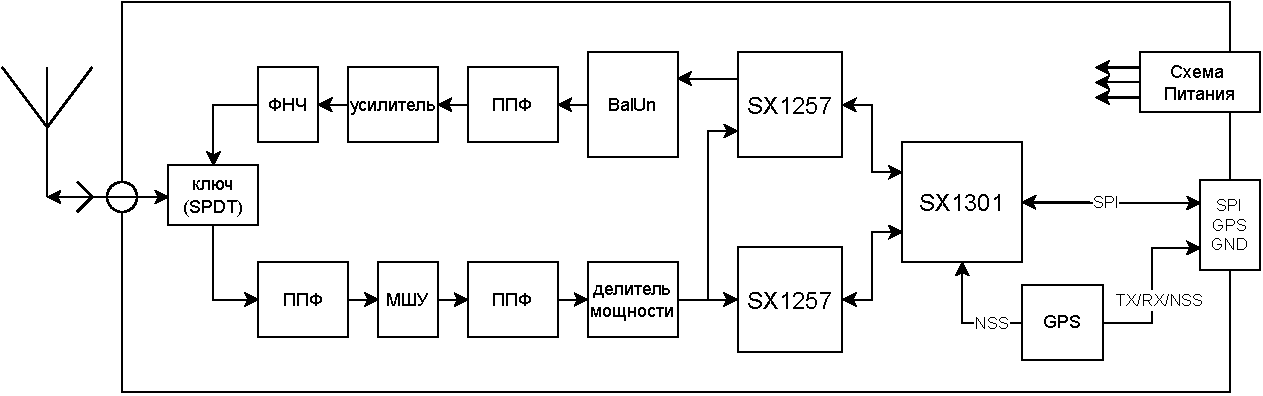
\includegraphics[width=0.9\textwidth,keepaspectratio]{BS-StructSch.pdf}
	\caption{Структурная схема БС}%
	\label{fig:BS-StructSch}
\end{figure}


\subsection{Выбор ЭКБ}
Исходя из составленной структурной схемы был произведён подбор электронной компонентной базы для БС.

\subsubsection{Выбор ППФ}

В диапазоне УКВ широкое распространение получили фильтры на поверхностных акустических волнах (ПАВ). Это обусловлено их высокими электрическими характеристиками (малые потери, малый коэффициент прямоугольности и высокая избирательность фильтра) при малых габаритных размерах. Кроме того, фильтры на ПАВ более устойчивы к внешним воздействующим факторам по сравнению с аналогами.

Исходя из стоимости, доступности, качества и количества предоставляемой производителем информации об устройстве, был выбран фильтр ФП3П7-814-10 производства Бутис-М. Производитель рекомендует его для применения в устройствах сетей LoRaWAN. Его размеры составляют 3х3х1,5 мм, а основные характеристики приведены на Рисунках \ref{fig:SAW-filter-graph-pass} и \ref{fig:SAW-filter-graph-VSWR}

\begin{figure}[H]
	\centering
	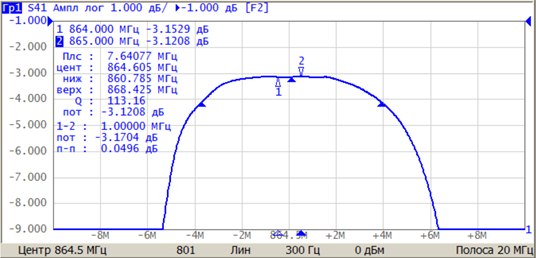
\includegraphics[width=0.8\textwidth,keepaspectratio]{SAW-filter-graph-pass.png}
	\caption{Передаточная характеристика фильтра ФП3П7-814-10}%
	\label{fig:SAW-filter-graph-pass}
\end{figure}

\begin{figure}[H]
	\centering
	\begin{subfigure}[b]{0.49\textwidth}
		\centering
		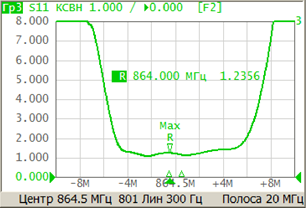
\includegraphics[width=\textwidth]{SAW-filter-graph-VSWR1.png}
		\caption{}%
		\label{fig:SAW-filter-graph-VSWR1}
	\end{subfigure}
	\hfill
	\begin{subfigure}[b]{0.49\textwidth}
		\centering
		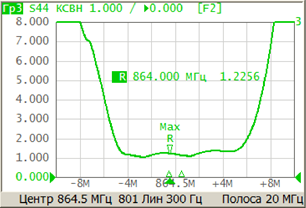
\includegraphics[width=\textwidth]{SAW-filter-graph-VSWR2.png}
		\caption{}%
		\label{fig:SAW-filter-graph-VSWR2}
	\end{subfigure}
	\caption{%
		КСВН фильтра ФП3П7-814-10
		(а) по входу и
		(б) по выходу 
	}%
	\label{fig:SAW-filter-graph-VSWR}
\end{figure}

\subsubsection{Выбор ФНЧ}
На роль ФНЧ был выбран фильтр 0868LP15A020 производства Johanson Technology. Его размеры составляют 2х1,25х1 мм, а основные характеристики приведены на Рисунке \ref{fig:LPF-graph}.

\begin{figure}[H]
	\centering
	\begin{subfigure}[b]{0.49\textwidth}
		\centering
		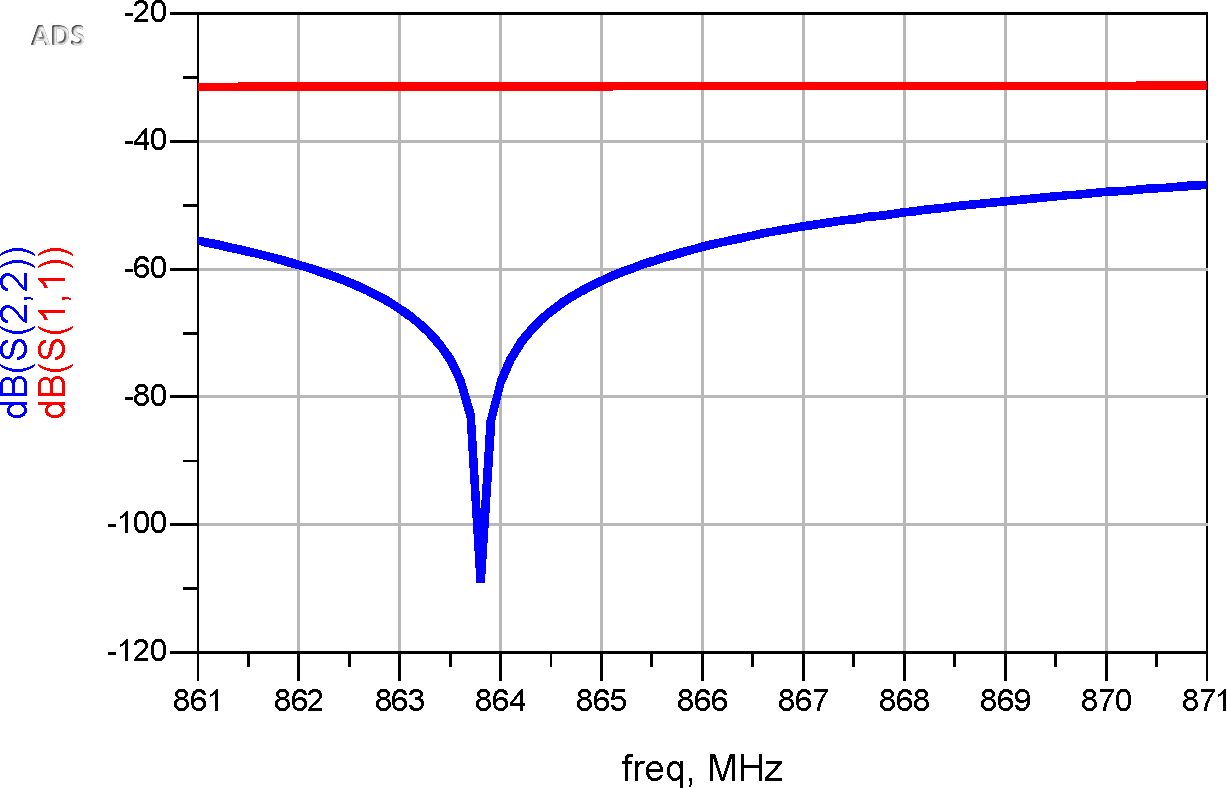
\includegraphics[width=\textwidth]{LPF-graph1122.pdf}
		\caption{}%
		\label{fig:LPF-graph1122}
	\end{subfigure}
	\hfill
	\begin{subfigure}[b]{0.49\textwidth}
		\centering
		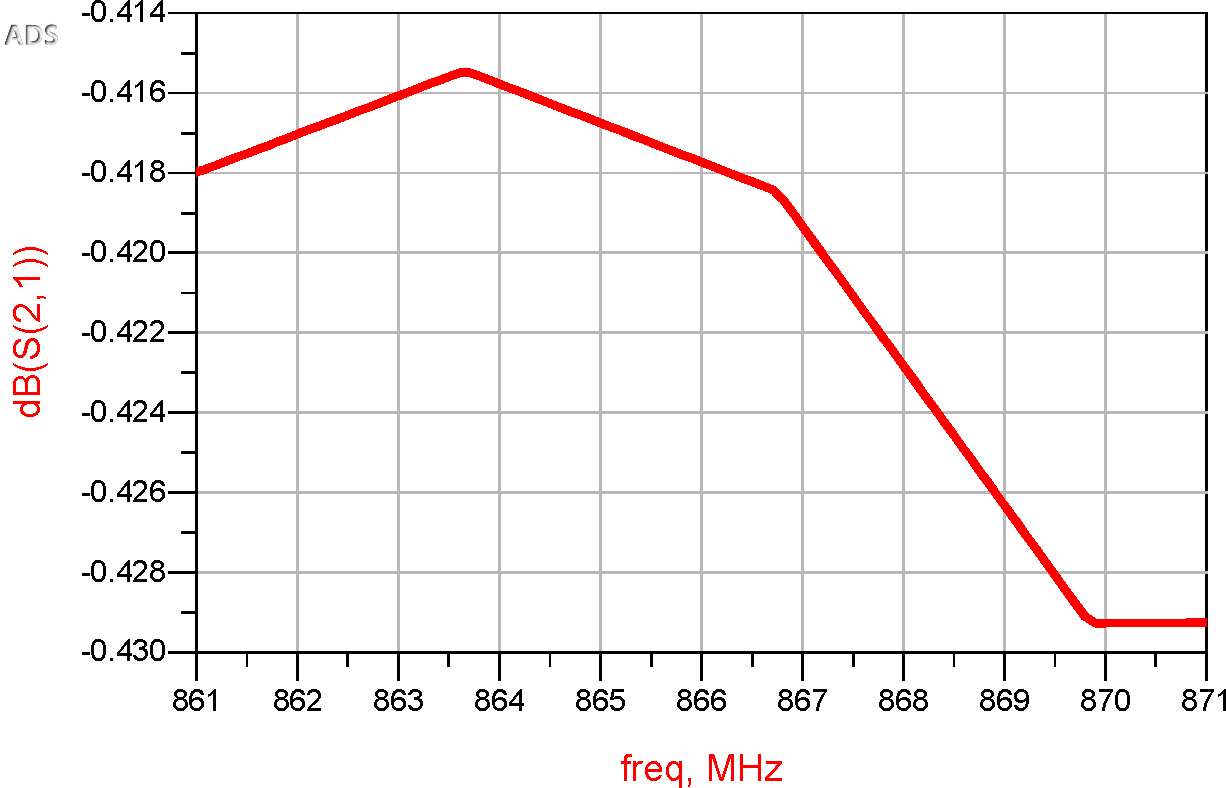
\includegraphics[width=\textwidth]{LPF-graph21.pdf}
		\caption{}%
		\label{fig:LPF-graph21}
	\end{subfigure}
	\caption{%
		КСВН фильтра ФП3П7-814-10
		(а) по входу и
		(б) по выходу 
	}%
	\label{fig:LPF-graph}
\end{figure}


\subsubsection{Выбор симметрирующего трансформатора}
В качестве симметрирующего трансформатора был выбран чип  \linebreak 0868BM15C0001 с размерами 2х1,25х1 мм. Его основные характеристики приведены на рисунках \ref{fig:balun-graph-SP} и \ref{fig:balun-graph-dirdif}.

\begin{figure}[H]
	\centering
	\begin{subfigure}[b]{0.49\textwidth}
		\centering
		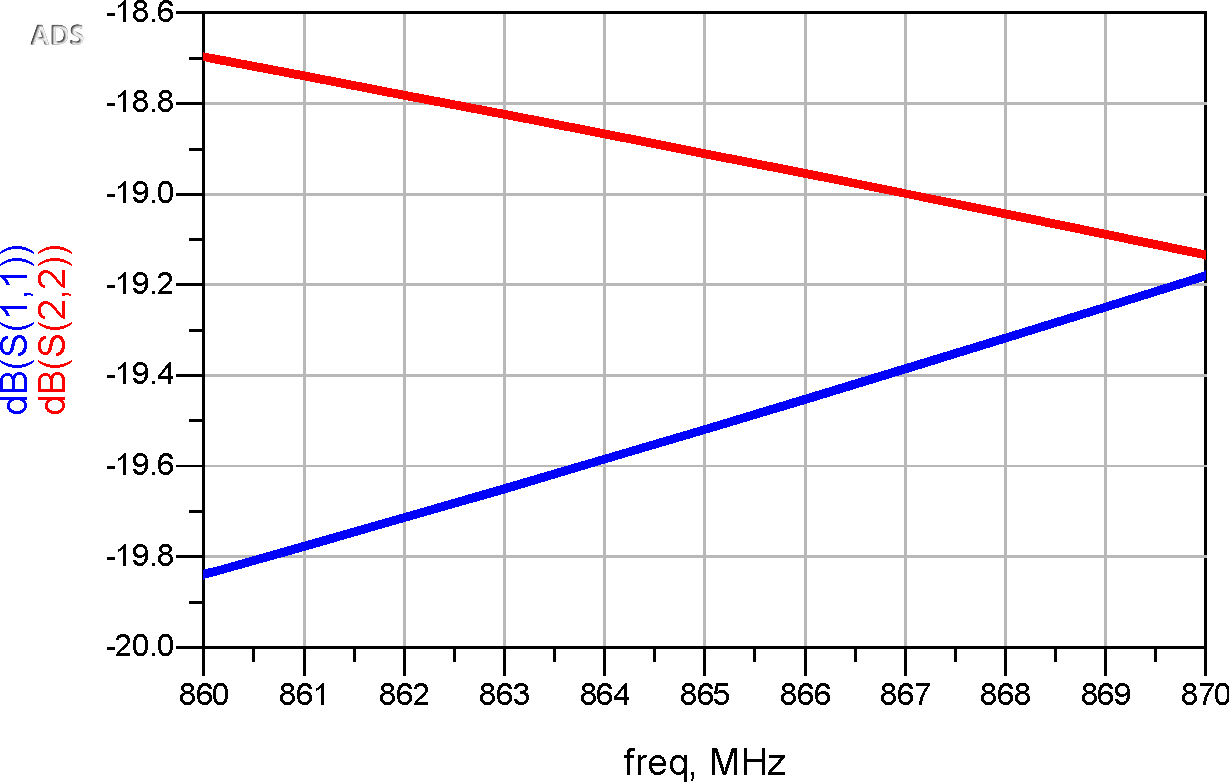
\includegraphics[width=\textwidth]{balun-graph-SP1122.pdf}
		\caption{}%
		\label{fig:balun-graph-SP1122}
	\end{subfigure}
	\hfill
	\begin{subfigure}[b]{0.49\textwidth}
		\centering
		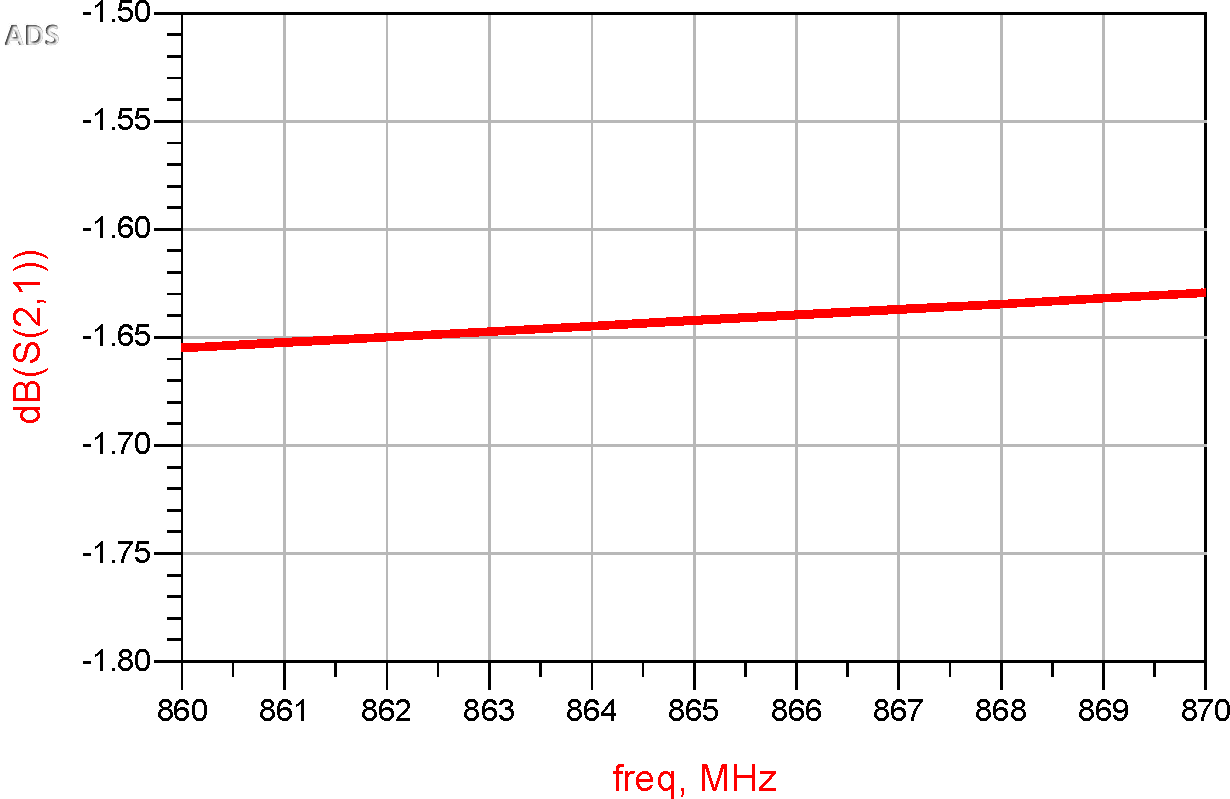
\includegraphics[width=\textwidth]{balun-graph-SP21.pdf}
		\caption{}%
		\label{fig:balun-graph-SP21}
	\end{subfigure}
	\caption{%
		Характеристики симметрирующего трансформатора 0868BM15C000
		(а) Коэффициенты отражения (дБ)
		(б) коэффициент передачи (дБ) 
	}%
	\label{fig:balun-graph-SP}
\end{figure}


\begin{figure}[H]
	\centering
	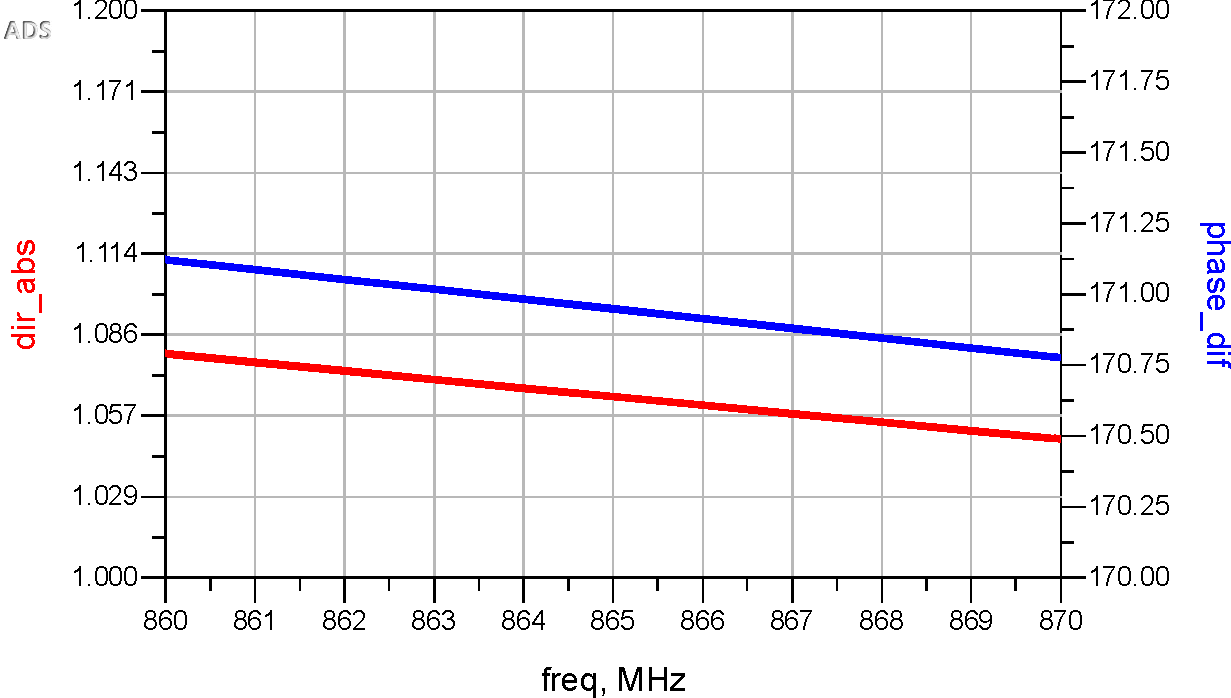
\includegraphics[width=0.8\textwidth,keepaspectratio]{balun-graph-dirdif.pdf}
	\caption{ Направленность (отношение амплитуд) и разница фаз балансных портов симметрирующего трансформатора 0868BM15C0001}%
	\label{fig:balun-graph-dirdif}
\end{figure}

\subsubsection{Выбор МШУ}

Для уменьшения коэффициента шума и улучшения чувствительности приёмного тракта требуется малошумящий усилитель. На его роль был выбран SPF5043Z производства Qorvo. Его основные параметры в необходимой полосе частот сведены в Таблице \ref{table:LNA-parameters}.

\begin{longtblr}[
	caption = {Основные параметры SPF5043Z},
	label = {table:LNA-parameters}
	]{
		colspec={Q[1,l,m]Q[1,l,m]},width=\textwidth,
		vlines,hlines,
		vspan=even,
		rowhead=1,
		row{1}={font=\bfseries}
	}
	%%%%%%%%%%%%%%%%%%%%%%%%%%%%%%%%%%%%%%%%%%%%%%%
	Параметр & Значение \\
	%%%%%%%%%%%%%%%%%%%%%%%%%%%%%%%%%%%%%%%%%%%%%%%%
	Усиление & 18,2 дБ \\
	Коэффициент шума & 0,7 дБ \\
	Точка однодецибельной компрессии & 22,6 дБмВт \\
	Размеры ШхДхВ & 2х2х1 мм \\
\end{longtblr}

\subsubsection{Выбор усилителя мощности}

Максимальная выходная мощность SX1257 равна -5 дБмВт. Для соответствия ТЗ требуется выходной усилитель мощности. Исходя из низкой стоимости, высокой эффективности и возможности регулирования усиления от 5 до 32 дБ был выбран усилитель RFPA0133 производства Qorvo. 

\subsubsection{Выбор опорных генераторов}

Для работы приемопередатчиков и процессора обработки данных требуются точные опорные генераторы. На их роль были выбраны KT2520K.32000. A.C.W.33.T.AS производства Kyocera и DSC1001CI2-133.0000 производства Microchip.

\subsubsection{Выбор ключа}

Выбираемый ключ должен иметь схему управления соответствующую SX1301, а именно - один управляющий сигнал выбирает рабочий порт, а другой разрешает или запрещает передачу сигнала. Данным параметрам соответствует RFSW1012. Его основные параметры показаны в таблице \ref{table:RFSW1012}

\begin{longtblr}[
	caption = {Основные gараметры выбранного ключа.},
	label = {table:RFSW1012}
	]{
		colspec={Q[1,l,m]Q[1,l,m]},width=\textwidth,
		vlines,hlines,
		vspan=even,
		rowhead=1,
		row{1}={font=\bfseries}
	}
	%%%%%%%%%%%%%%%%%%%%%%%%%%%%%%%%%%%%%%%%%%%%%%%
	Параметр & Значение \\
	%%%%%%%%%%%%%%%%%%%%%%%%%%%%%%%%%%%%%%%%%%%%%%%%
	Входные потери & 0,35 дБ \\
	Изоляция портов 1-2 & 48 дБ \\
	Диапазон частот & 5-6000 МГц \\
	Размеры (ШхДхВ) & 2х2х0,5 мм \\
\end{longtblr}

\subsubsection{Выбор GPS модуля.}

Для синхронизации времени и местоположения с сетью требуется информация о геолокации. Модуль uBlox Max7-Q имеет размеры (ШхДхВ) \linebreak 9,7х10,1х2,5 мм. Он поддерживает системы GPS и ГЛОНАСС, может определять местоположение с точностью до 2  м и имеет отдельный выход для генерации сигнала точного времени.

\subsection{Разработка подсистемы питания.}

Планируется питание от распространенных 9/12В блоков питания с штырьковым разъемом. В Таблице \ref{table:voltage-consumtion} показано потребление используемых устройств.

\begin{longtblr}[
	caption = {},
	label = {table:voltage-consumtion}
	]{
		colspec={Q[3,l,m]Q[4,l,m]Q[3,l,m]Q[6,l,m]},width=\textwidth,
		vlines,hlines,
		vspan=even,
		rowhead=1,
		row{1}={font=\bfseries}
	}
	%%%%%%%%%%%%%%%%%%%%%%%%%%%%%%%%%%%%%%%%%%%%%%%
	Устройство & Напряжение & Значение, В & Сила тока, макс, мА \\	
	%%%%%%%%%%%%%%%%%%%%%%%%%%%%%%%%%%%%%%%%%%%%%%%%
	\SetCell[r=2]{l} SX1301 
	& Питания портов & 3,3 & 10 \\
	& Питания ядра & 1,8 & 750 \\
	
	SX1257 & Питания & 3,3 & 85 \\
	
	VCXO & Питания & 3,3 & 2 \\
	
	\SetCell[r=2]{l} RFPA0133
	
	& Питания 1,2 & 3,6 & 250 \\
	& Смещения & 3 & 0,2 \\
	 
	SPF5043 & Питания & 5 & 100 \\
	
	RFSW1012 & Питания & 2,7-5,5 & 0,2 \\
	
	MAX7-Q & Питания & 3,3 & 67 \\	
\end{longtblr}

Формирование напряжения питания обеспечивается импульсными и линейными стабилизаторами напряжения. Первые нужны для высокоэффективного понижения напряжения, а вторые для устранения помех, создаваемыми в процессе их работы. На рисунке \ref{fig:BS-PowerSch} показана структурная схема подсистемы питания

\begin{figure}[H]
	\centering
	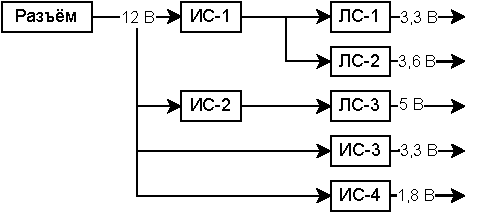
\includegraphics[width=0.8\textwidth,keepaspectratio]{BS-PowerSch.pdf}
	\caption{Структурная схема подсистемы питания БС}%
	\label{fig:BS-PowerSch}
\end{figure}

\begin{itemize}
	\item Разъём выберем DS-201 – это штырьковый разъём-розетка 2,1х5,5мм
	\item В качестве импульсных стабилизаторов будет применяться ST1S14PH производства STMicroelectronics – это стабилизатор с диапазоном входных напряжений от 5.5 до 48 В и выходным током до 3 А. Выходное напряжение регулируется с помощью резистивного делителя, рассчитываемого по формуле 
	\begin{equation}
		\label{eq:stab-voltage-output}
		V_{out}=1,22\cdot(1+R1/R2)
	\end{equation}
	Схема включения изображена на рисунке \ref{fig:ST1S14PH-PS}
	\begin{figure}[H]
		\centering
		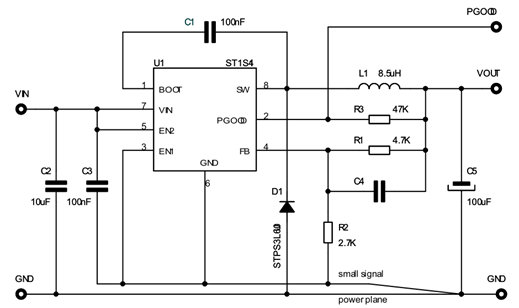
\includegraphics[width=0.8\textwidth,keepaspectratio]{ST1S14PH-PS.png}
		\caption{Типичная схема включения ST1S14PH}%
		\label{fig:ST1S14PH-PS}
	\end{figure}
	
	\item На роль линейных стабилизаторов был выбран LT1965EDD – это стабилизатор с диапазоном входных напряжений от 1,8 до 20 В, максимальным выходным током 1,1 А и падением напряжения 310 мВ. Выходное напряжение регулируется с помощью резистивного делителя, рассчитываемого по формуле \ref{eq:stab-voltage-output}.

	Схема включения изображена на рисунке \ref{fig:LT1965EDD-PS}.

	\begin{figure}[H]
		\centering
		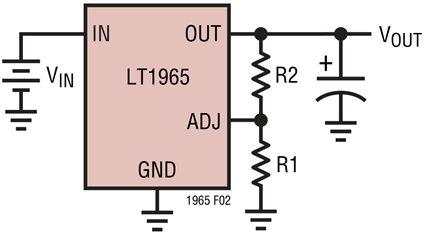
\includegraphics[width=0.8\textwidth,keepaspectratio]{LT1965EDD-PS.png}
		\caption{Типичная схема включения LT1965EDD-PS}%
		\label{fig:LT1965EDD-PS}
	\end{figure}
\end{itemize}

\subsection{Системное моделирование.}
Выполним моделирование каждого компонента по отдельности, а также входной и выходной цепи.

Моделирование каждого элемента выполняется поочередно в двух режимах – схемном и симуляционном. В первом для расчётов используются идеальные линии передачи, во втором строится  участок платы, включающий посадочное место устройства, сигнальные линии и линии питания, а также необходимые схемы согласования, и проводится моделирование с помощью ЕМ-симулятора.

Для уменьшения размеров устройства каждый блок будет согласован не с 50-тиомной линией, а с соседним блоком, таким образом моделирование цепи будет выполняться следующим образом: вход первого устройства согласуется с 50-тиомной линией, а сопротивление выходного порта приравнивается к выходному сопротивлению устройства, сопротивление входного порта следующего блока приравнивается к выходному сопротивлению предыдущего и согласуется с входным сопротивлением устройства; последний же блок согласуется по входу с предыдущим блоком, а по выходу - с 50-тиомной линией.

Рассчитаем общую для всего устройства ширину 50-тиомной линии с помощью утилиты TxLine. Параметры платы и линий будут задаваться с учётом технологических возможностей современных производств.

\begin{figure}[H]
	\centering
	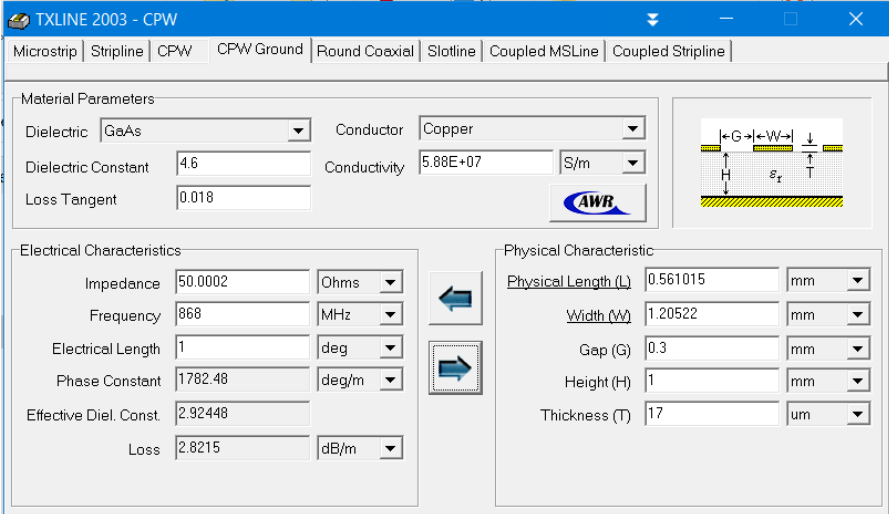
\includegraphics[width=0.8\textwidth,keepaspectratio]{BS LineCalc.png}
	\caption{Расчёт ширины линии}%
	\label{fig:BS LineCalc}
\end{figure}

\subsubsection{Результаты моделирования передающего тракта.}
На Рисунке \ref{fig:OPL-sch} показано схемное представление передающего тракта БС. Каждый блок был согласован и промоделирован с помощью ЕМ-симулятора. Результаты моделирования всего тракта показаны на Рисунках \ref{fig:OPL-imp} и \ref{fig:OPL-VSWR-trans}.

\begin{figure}[H]
	\centering
	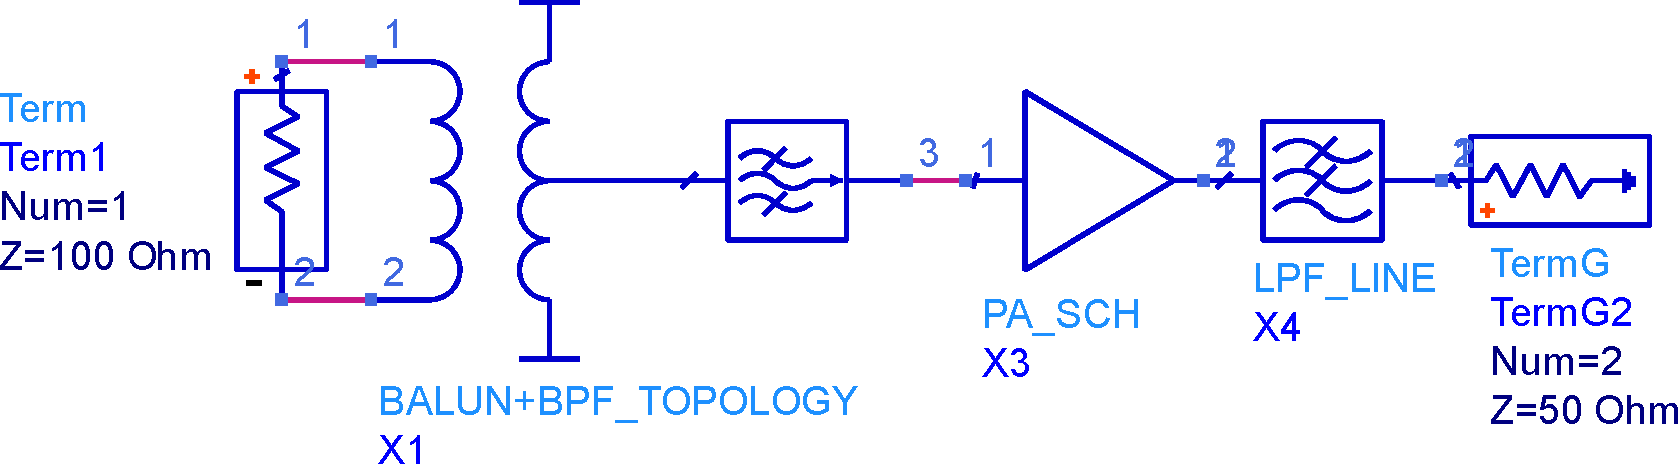
\includegraphics[width=\textwidth,keepaspectratio]{OPL-sch.pdf}
	\caption{Итоговая модель выходного тракта БС}%
	\label{fig:OPL-sch}
\end{figure}

\begin{figure}[H]
	\centering
	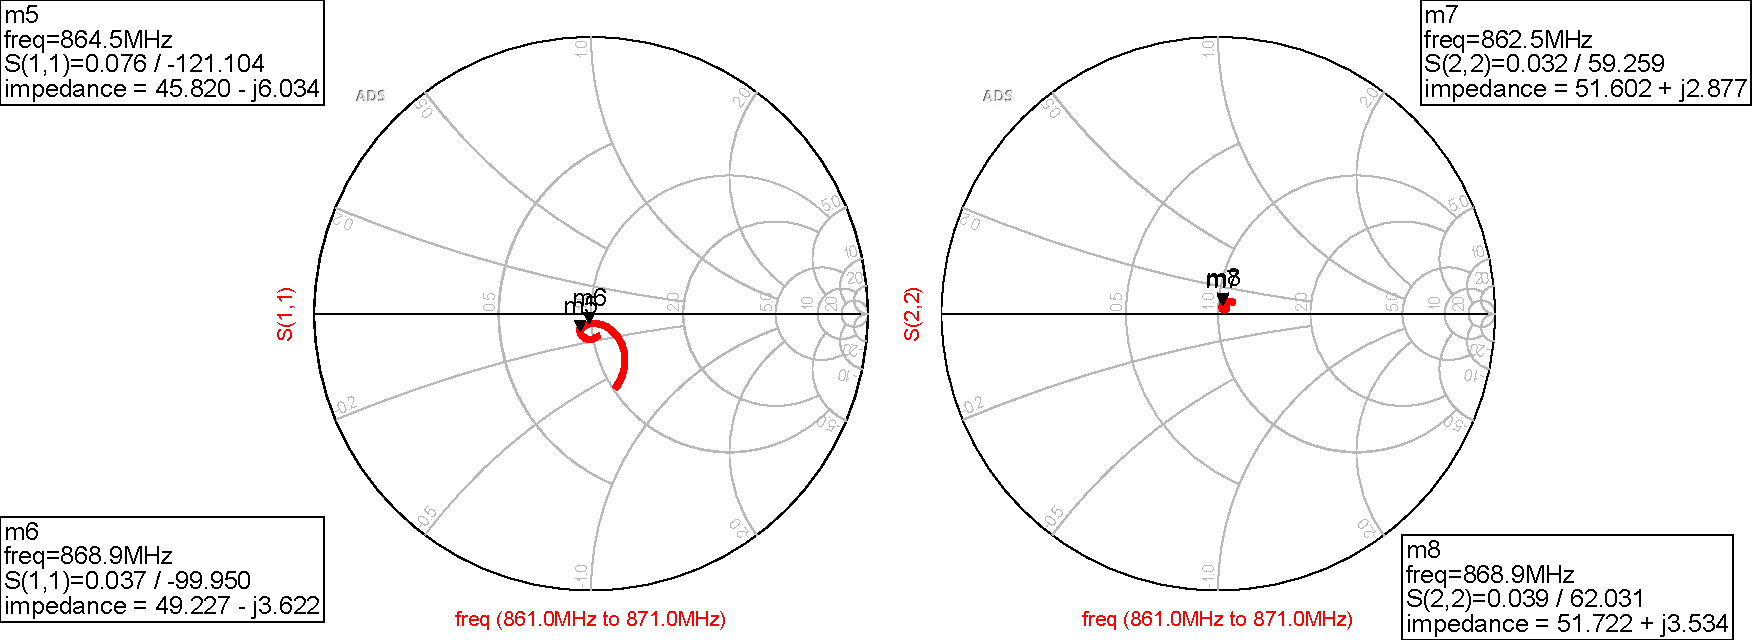
\includegraphics[width=\textwidth,keepaspectratio]{OPL-imp.pdf}
	\caption{входное и выходное сопротивление передающего тракта}%
	\label{fig:OPL-imp}
\end{figure}

\begin{figure}[H]
	\centering
	\begin{subfigure}[b]{0.49\textwidth}
		\centering
		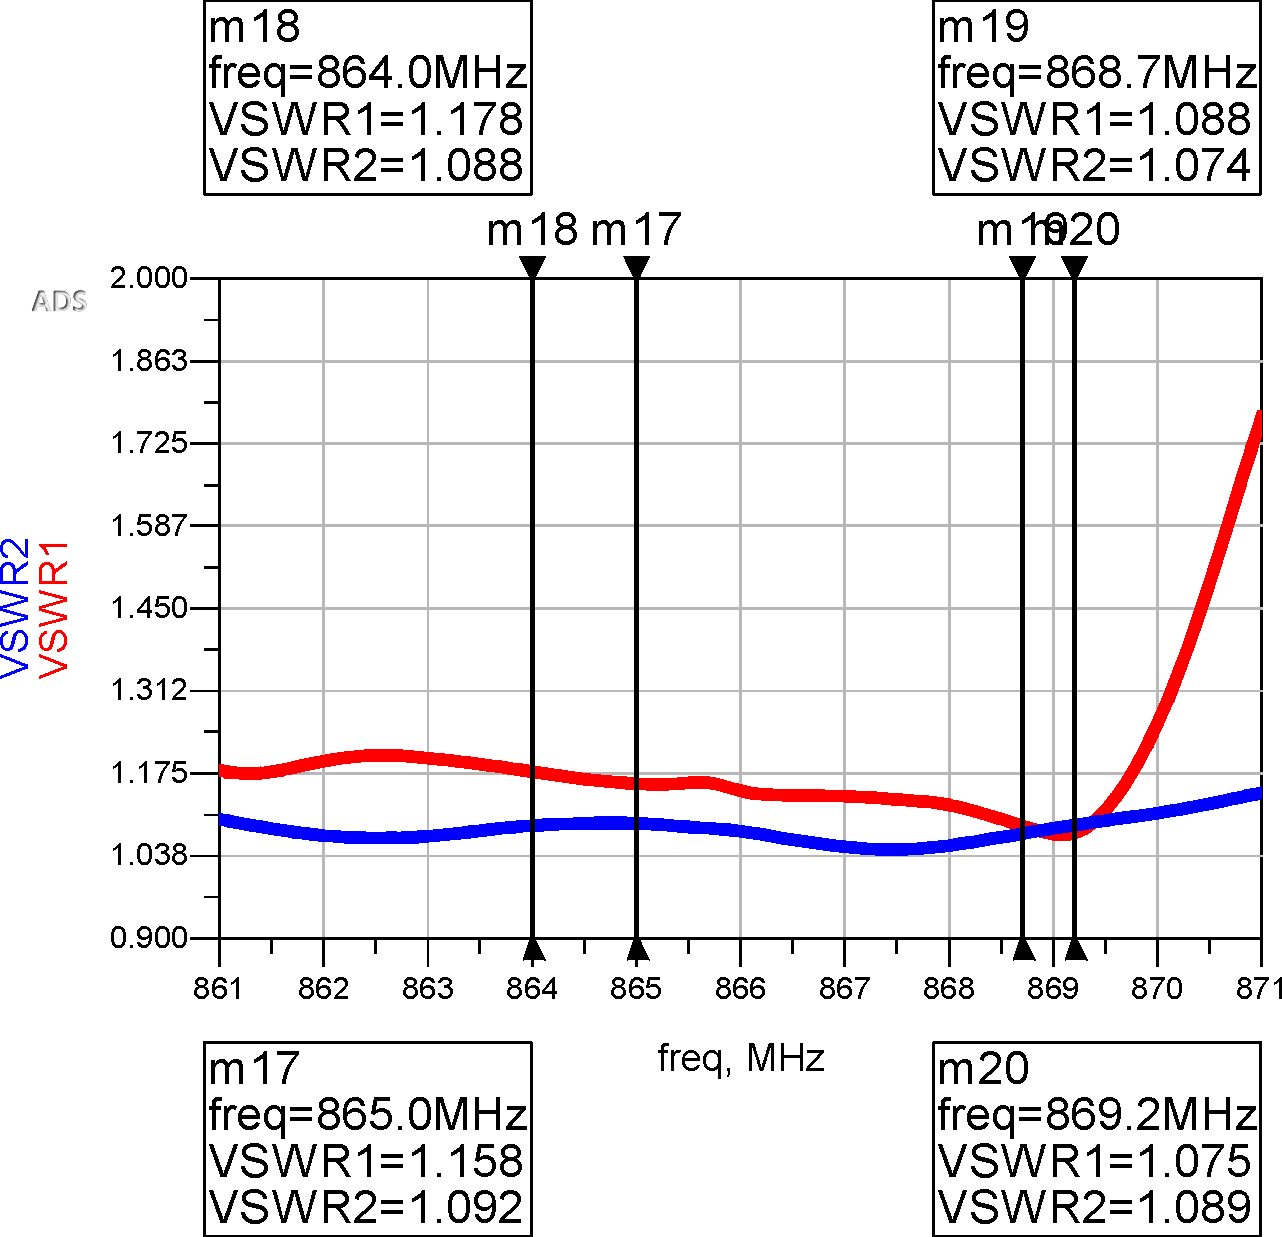
\includegraphics[width=\textwidth]{OPL-VSWR.pdf}
		\caption{}%
		\label{fig:OPL-VSWR}
	\end{subfigure}
	\hfill
	\begin{subfigure}[b]{0.49\textwidth}
		\centering
		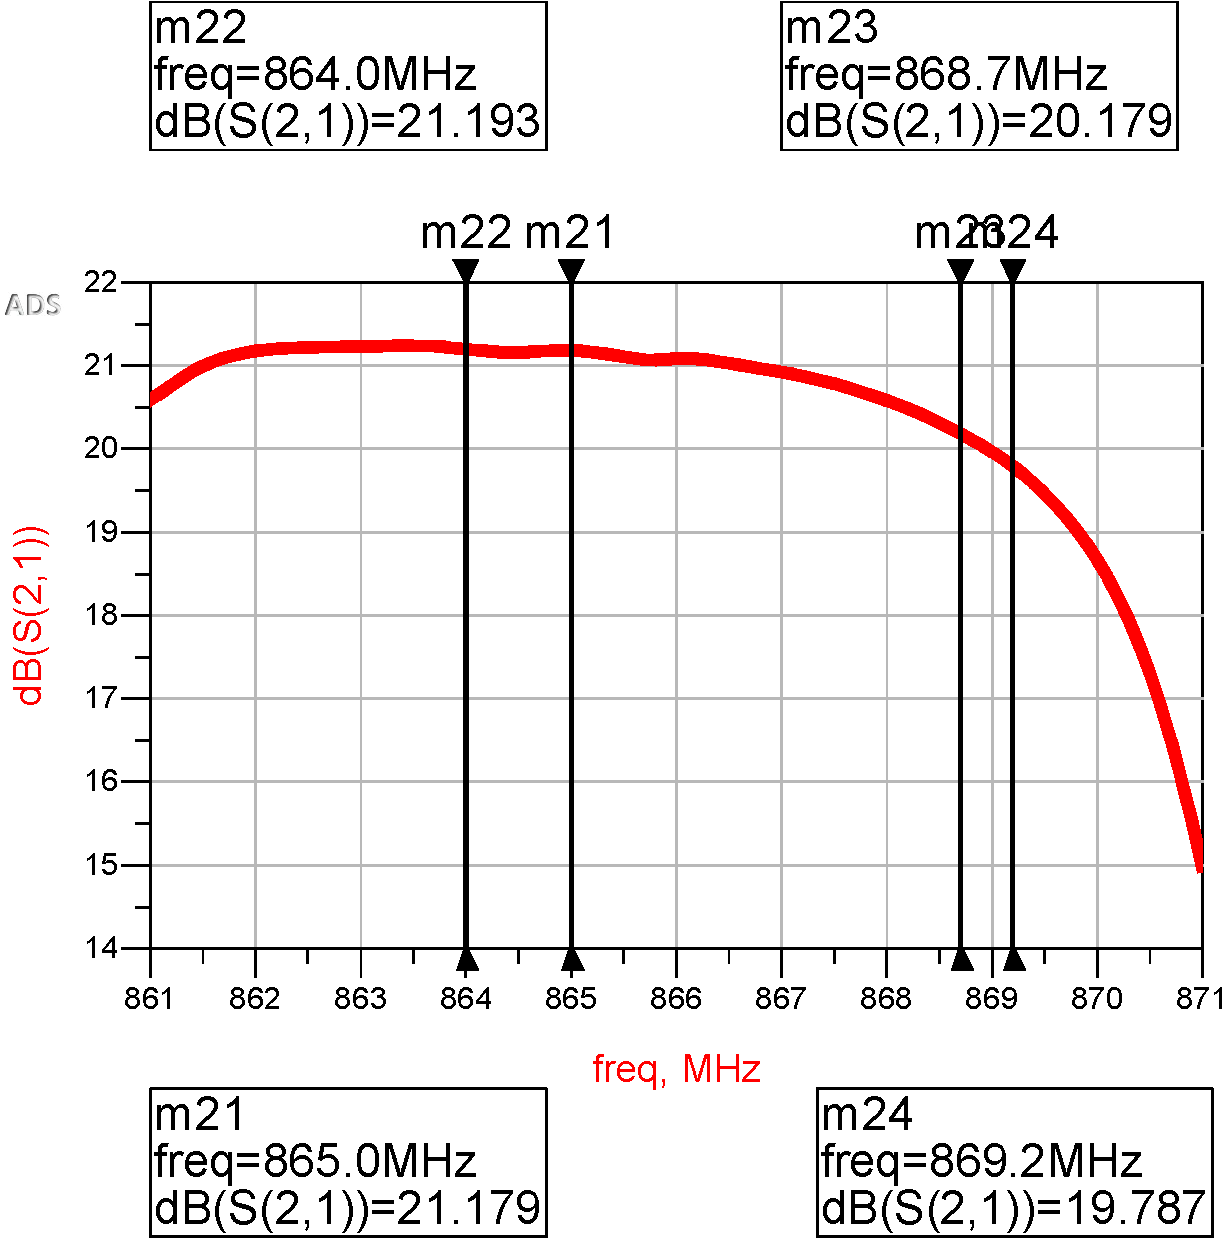
\includegraphics[width=\textwidth]{OPL-trans.pdf}
		\caption{}%
		\label{fig:OPL-trans}
	\end{subfigure}
	\caption{%
		(а) КСВН передающего тракта
		(б) Коэффициент передачи передающего тракта (дБ)
	}%
	\label{fig:OPL-VSWR-trans}
\end{figure}

На рисунке \ref{fig:OPL-trans} показано максимально возможное усиление в канале. Максимальная выходная мощность SX1257 равна -5 дБм, таким образом максимально возможная выходная мощность равна 16 дБм. С помощью программного регулирования можно устанавливать выходную мощность от  -7 до 16 дБм, таким образом требование к мощности передаваемого сигнала можно считать удовлетворенным.

Стоит, однако, отметить, что производитель выходного усилителя не предоставил файлов S-параметров, поэтому для моделирования использовался универсальный блок усилителя, параметры которого задавались исходя из имеющейся документации на элемент. Для более точного определения параметров элемента и более качественного его согласования была разработана измерительная плата, а для ускорения процесса производства на плате основного устройства будут размещены посадочные места для универсальной схемы согласования. Подробнее про разработку платы измерения параметров УМ рассказано в Главе \ref{sect:bs-oa-mes}.

\subsubsection{Результаты моделирования приемного тракта.}
Основной участок приёмного тракта необходимо спроектировать так, чтобы с одной стороны он был согласован с антенной, а с другой - с делителем мощности.

На Рисунке \ref{fig:IPL-sch} показано схемное представление передающего тракта БС. Каждый блок был согласован и промоделирован с помощью ЕМ-симулятора. Результаты моделирования всего тракта показаны на Рисунках \ref{fig:IPL-imp}, \ref{fig:IPL-VSWR-trans} и \ref{fig:IPL-NF}.

\begin{figure}[H]
	\centering
	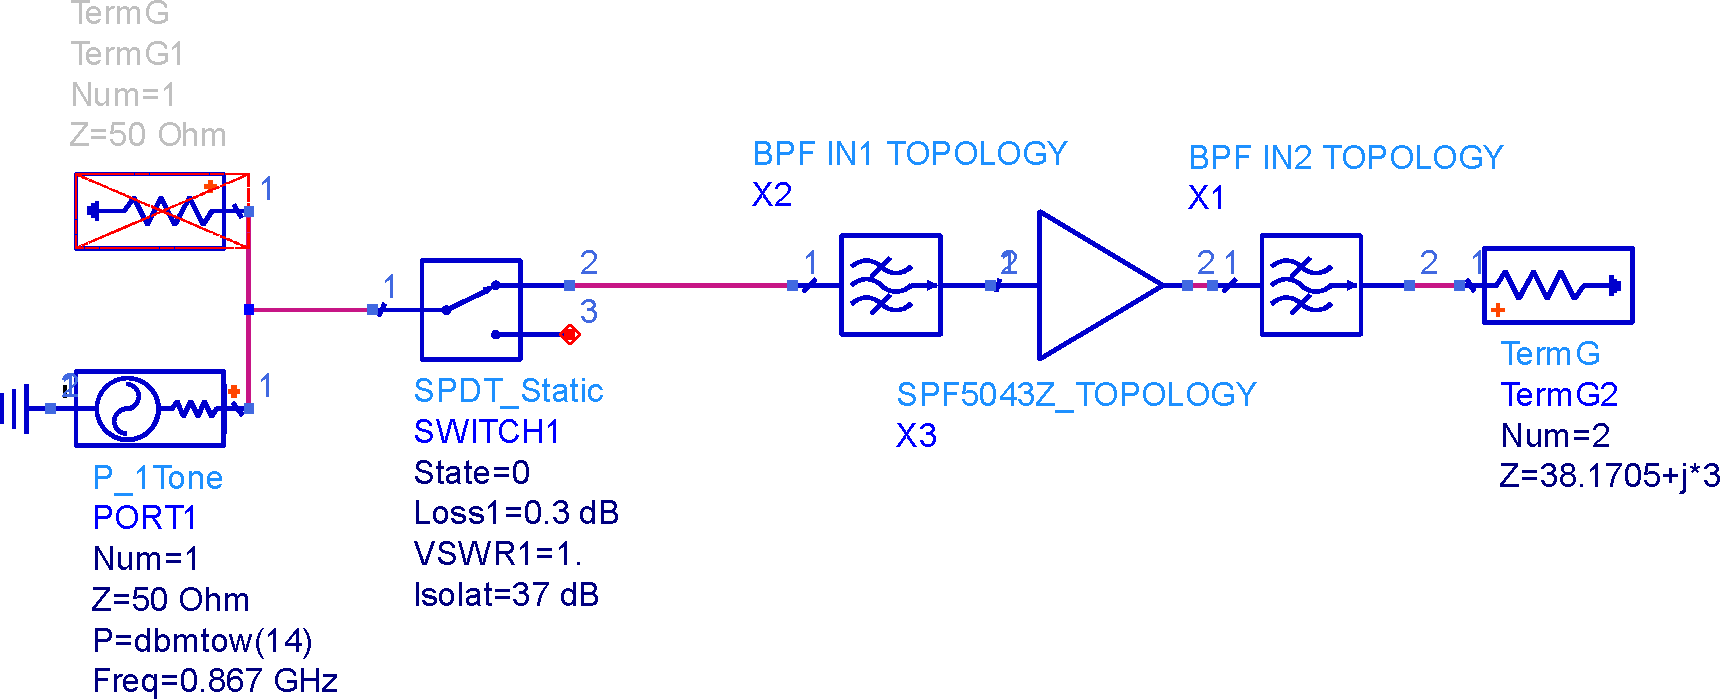
\includegraphics[width=\textwidth,keepaspectratio]{IPL-sch.pdf}
	\caption{Итоговая модель приемного тракта БС}%
	\label{fig:IPL-sch}
\end{figure}

\begin{figure}[H]
	\centering
	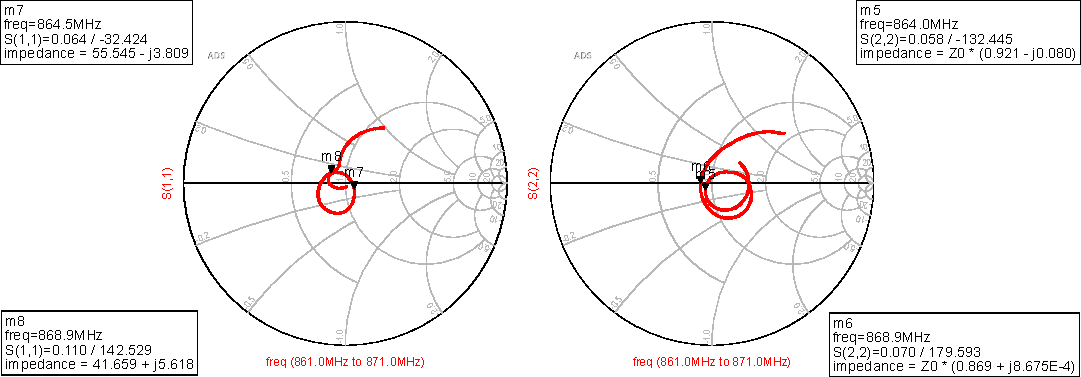
\includegraphics[width=0.9\textwidth,keepaspectratio]{IPL-imp.pdf}
	\caption{входное и выходное сопротивление приёмного тракта}%
	\label{fig:IPL-imp}
\end{figure}

\begin{figure}[H]
	\centering
	\begin{subfigure}[b]{0.49\textwidth}
		\centering
		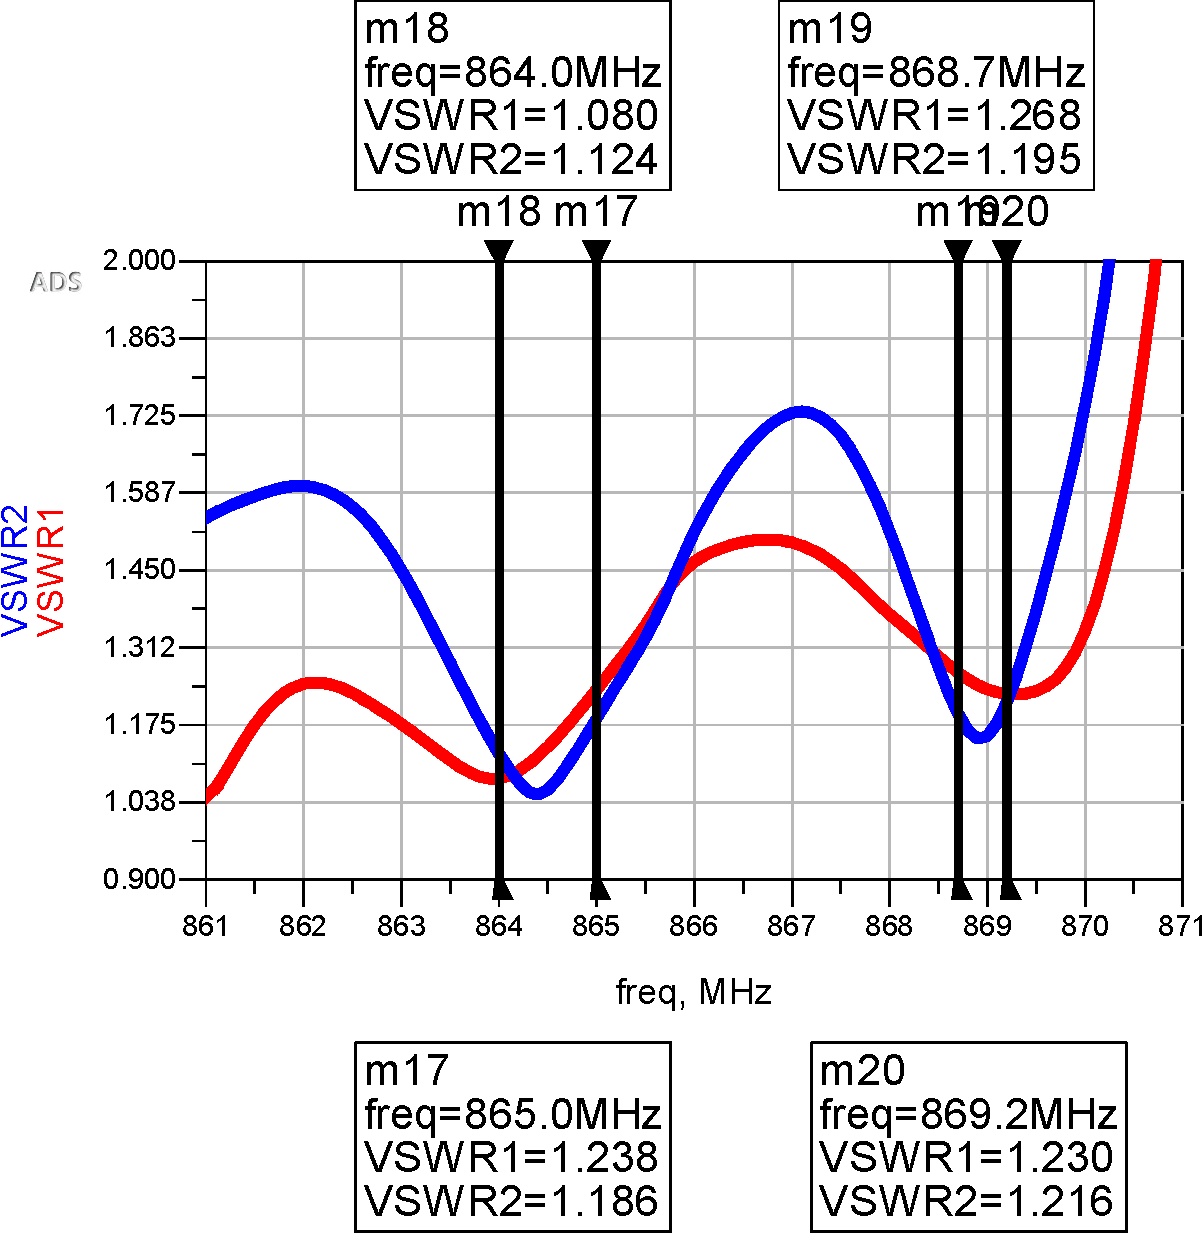
\includegraphics[width=\textwidth]{IPL-VSWR.pdf}
		\caption{}%
		\label{fig:IPL-VSWR}
	\end{subfigure}
	\hfill
	\begin{subfigure}[b]{0.49\textwidth}
		\centering
		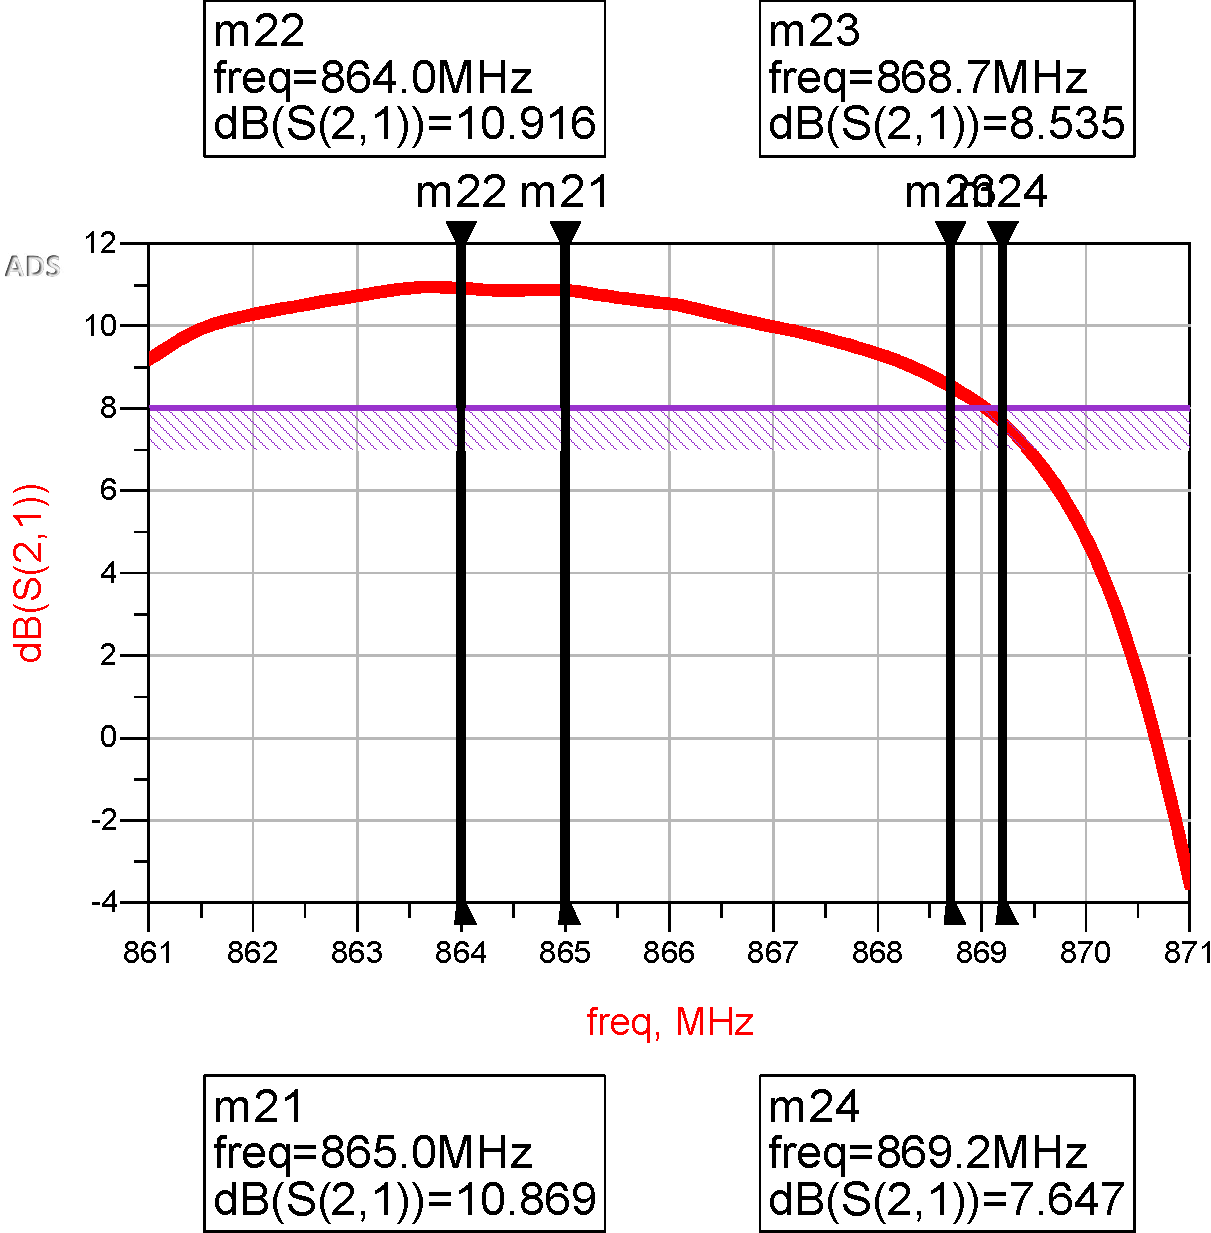
\includegraphics[width=\textwidth]{IPL-trans.pdf}
		\caption{}%
		\label{fig:IPL-trans}
	\end{subfigure}
	\caption{%
		(а) КСВН приёмного тракта
		(б) Коэффициент передачи приёмного тракта (дБ)
	}%
	\label{fig:IPL-VSWR-trans}
\end{figure}

\begin{figure}[H]
	\centering
	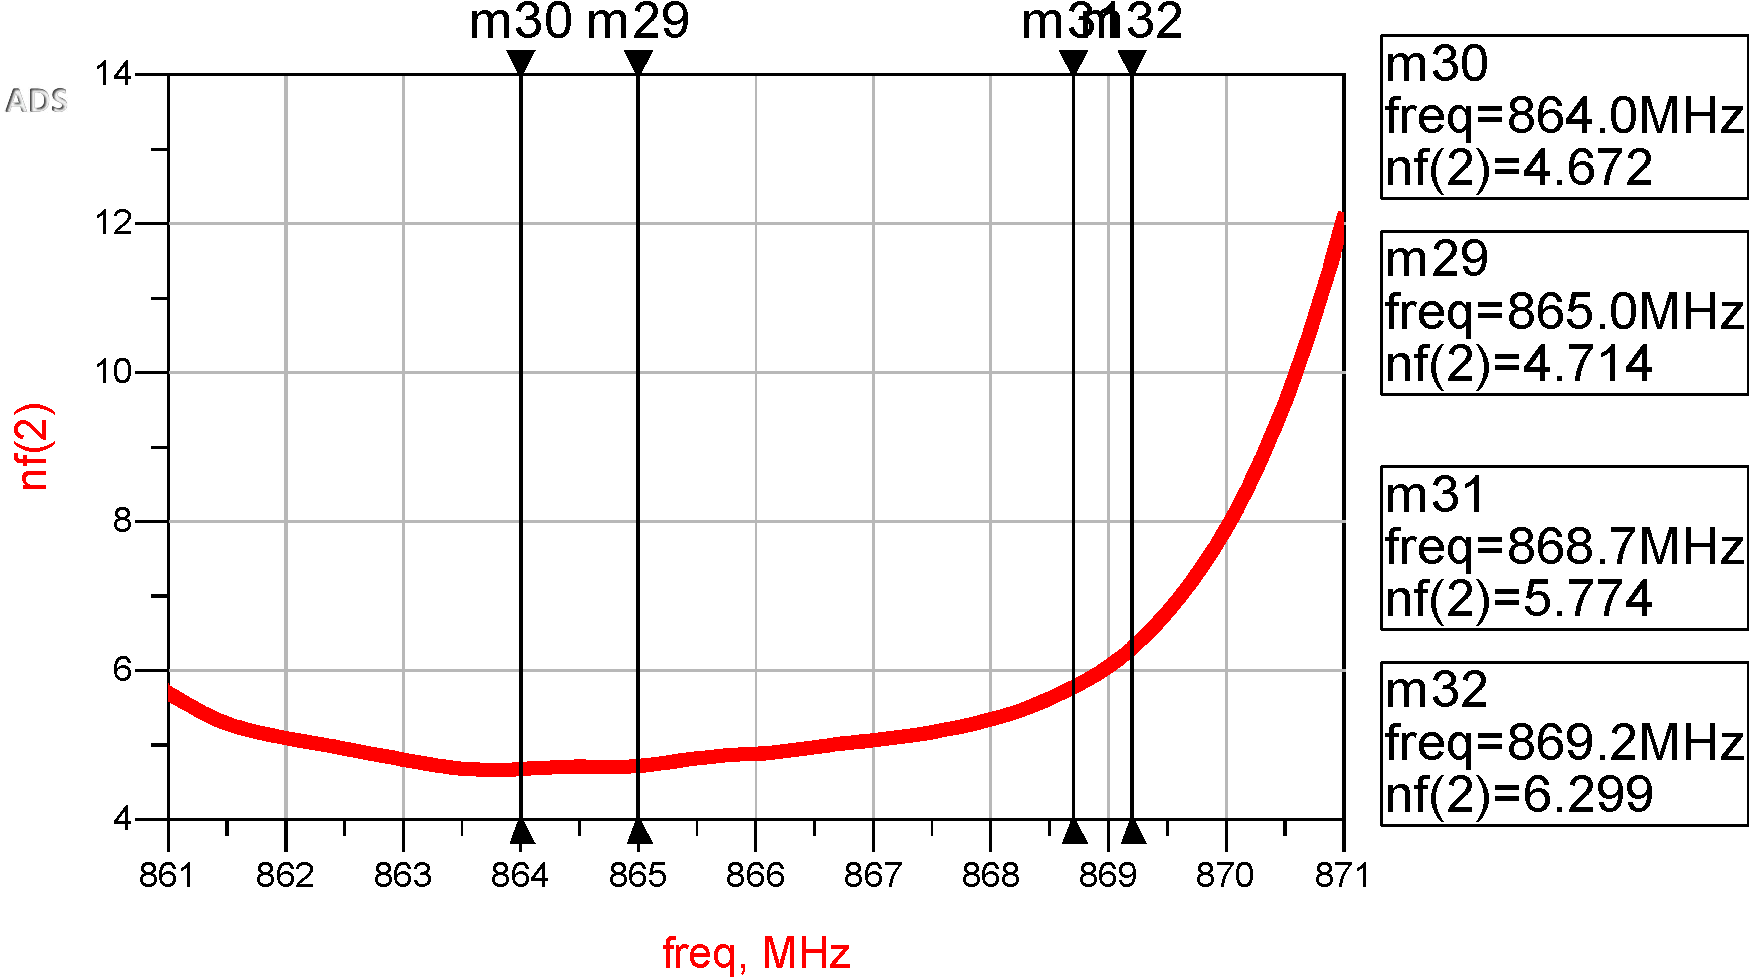
\includegraphics[width=0.75\textwidth,keepaspectratio]{IPL-NF.pdf}
	\caption{$K_\text{Ш}$ приемного тракта}%
	\label{fig:IPL-NF}
\end{figure}

Основываясь на полученных результатах произведем расчёт чувствительности устройства по формуле
\begin{equation}
	{Sensitivity}[\text{дБм}] = N[\text{дБм}]+{SNR}_\text{треб}[\text{дБ}]+NF-K_\text{п}+3
\end{equation}

Здесь N - мощность шума в выбранной полосе в дБм, ${SNR}_\text{треб}$ - требуемое отношение сигнал-шум в дБ, NF - коэффициент шума, $K_\text{п}$ - коэффициент передачи приемного тракта, дБ. 3 дБ необходимо прибавлять для учета деления мощности между приемопередатчиками. 

Расчёт чувствительности проводился для $f_c=869$~МГц, так как это позволяет оценить предельные возможности приемного тракта. Худшие показатели чувствительности достигаются при SF=6 и полосе 250~кГц. Требуемое отношение сигнал-шум в таком случае составляет -7.5 дБ. 
Экспортируем значения в переменные и рассчитаем чувствительность прямо в ADS. Расчёты и их результат показаны на Рисунке \ref{fig:IPL-sens-count}

\begin{figure}[H]
	\centering
	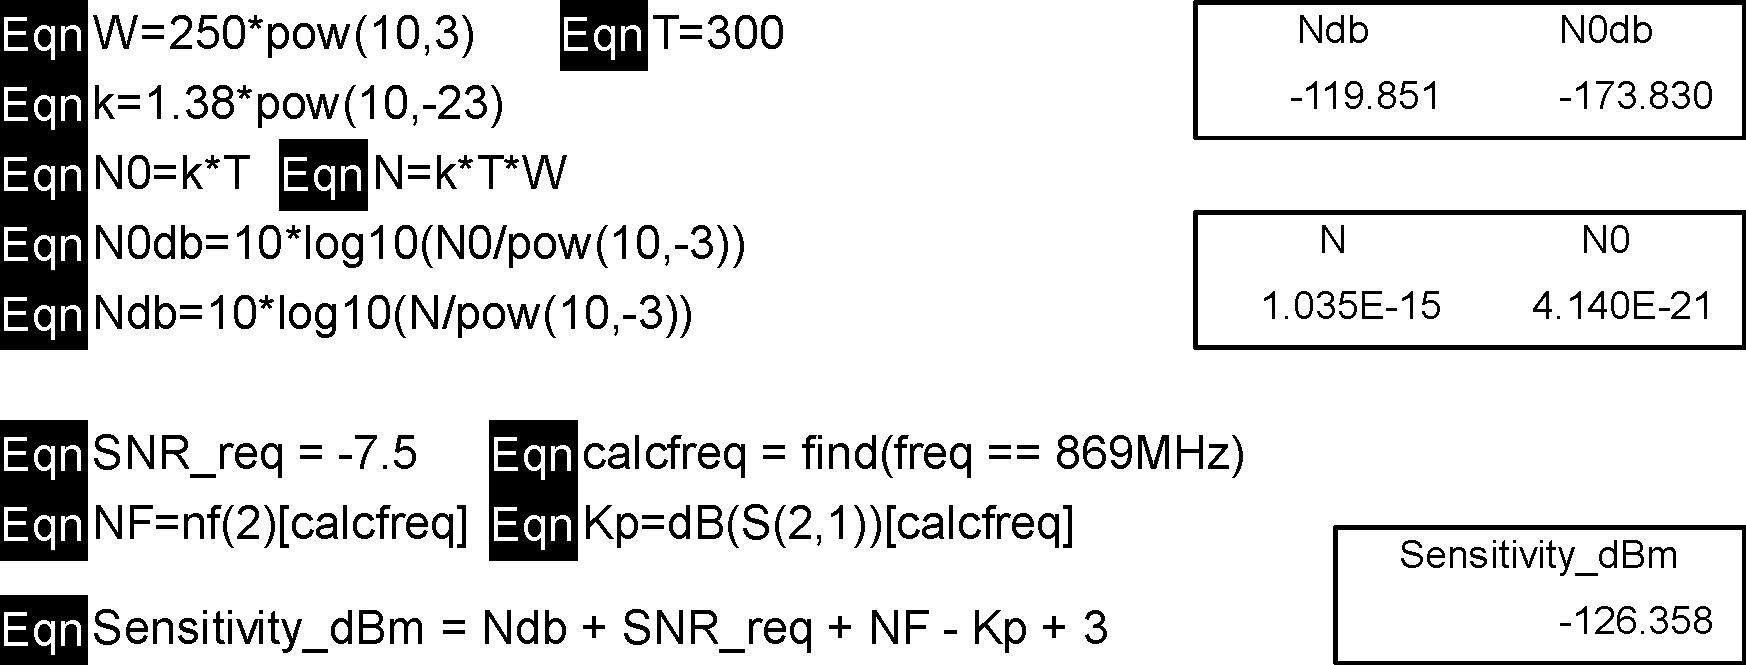
\includegraphics[width=\textwidth,keepaspectratio]{IPL-sens-count.pdf}
	\caption{Расчёт чувствительности приемного тракта БС}%
	\label{fig:IPL-sens-count}
\end{figure}

Рассчитанное значение чувствительности составляет минус 126 дБм, следовательно, ТЗ на приёмный тракт можно считать выполненным.

\subsubsection{Делитель мощности.}

Для увеличения возможностей параллельной многоканальной обработки данных необходимо разделять входной поток между двумя приемопередатчиками. Входное сопротивление SX1257 равно 50 Ом. Необходимо разработать и согласовать делитель мощности. На Рисунках \ref{fig:coupler-em} и \ref{fig:coupler-match} показаны топология и схема согласования делителя. 

\begin{figure}[H]
	\centering
	\begin{subfigure}[c]{0.49\textwidth}
		\centering
		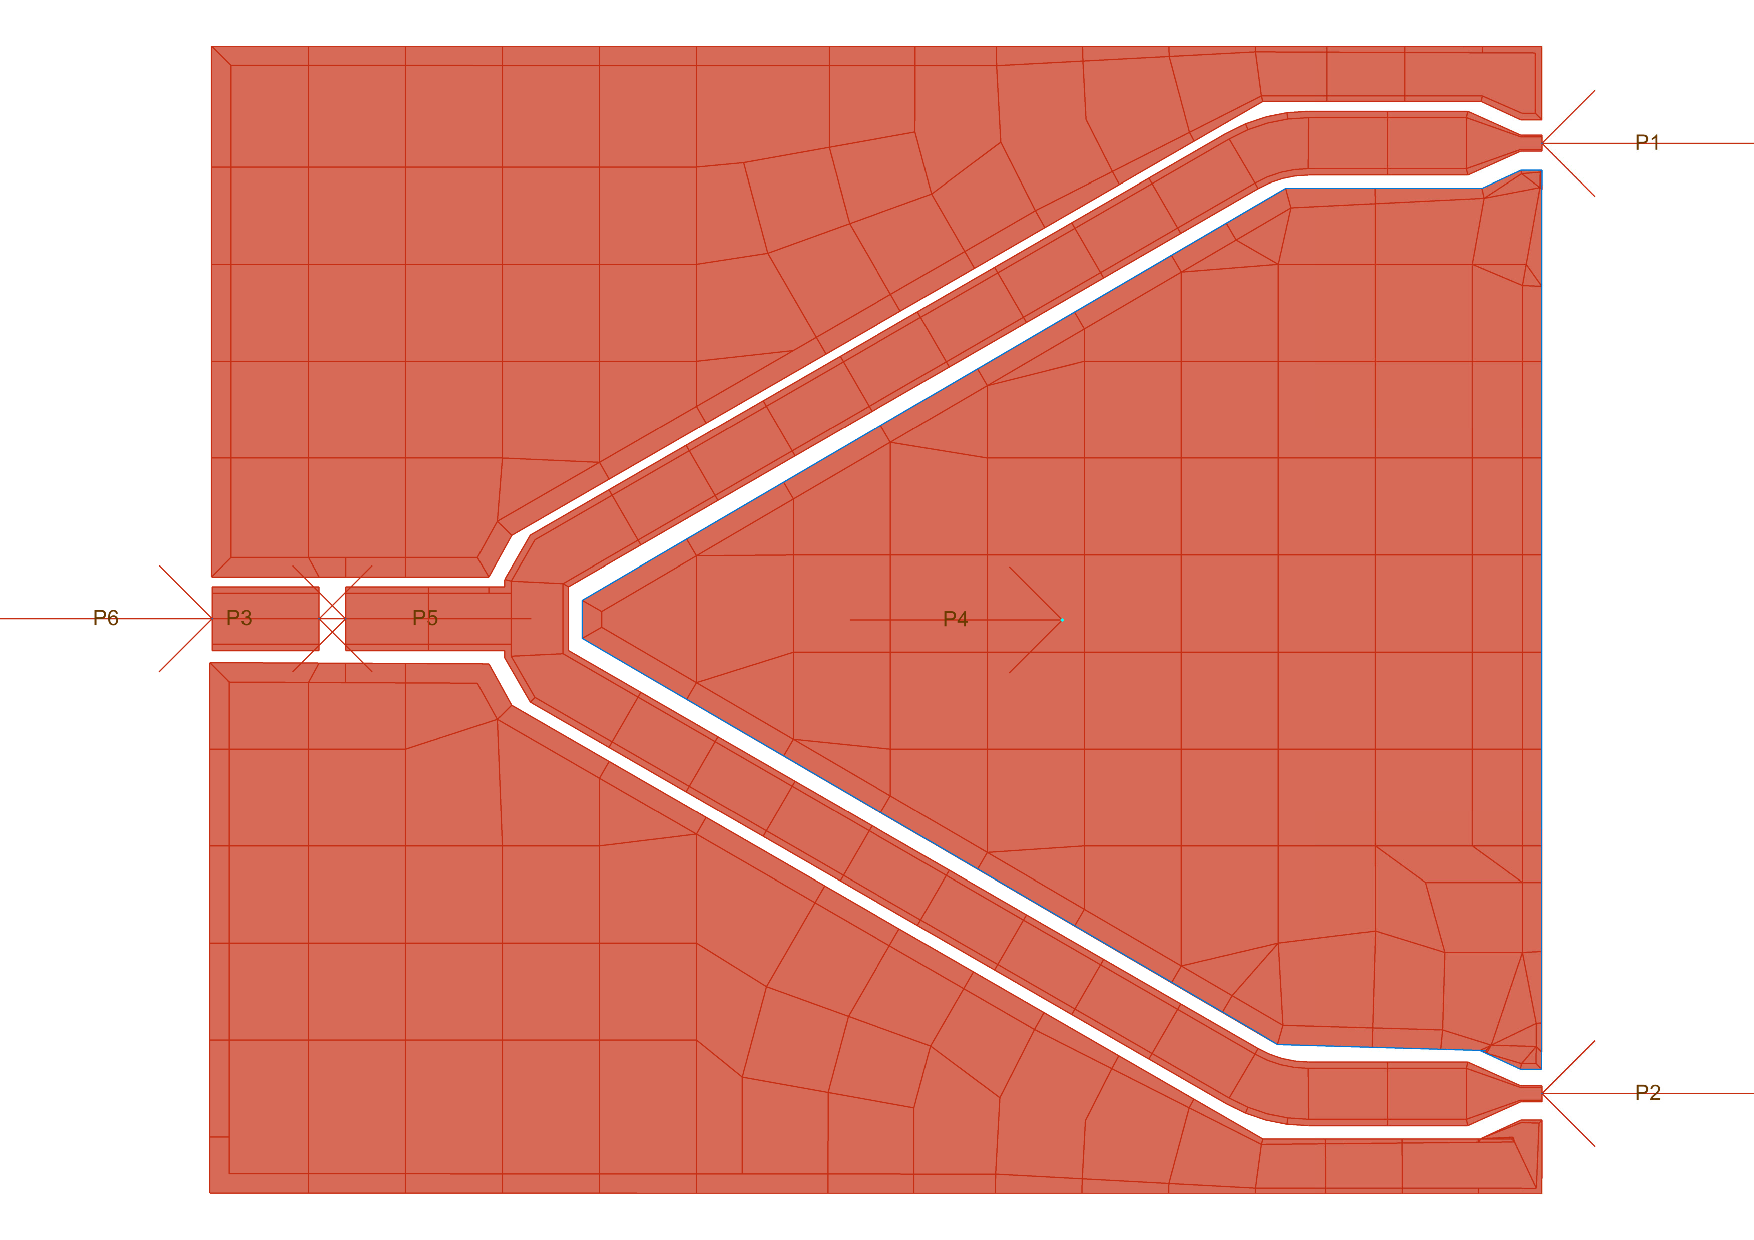
\includegraphics[width=\textwidth]{coupler-em.pdf}
		\caption{}%
		\label{fig:coupler-em}
	\end{subfigure}
	\hfill
	\begin{subfigure}[c]{0.49\textwidth}
		\centering
		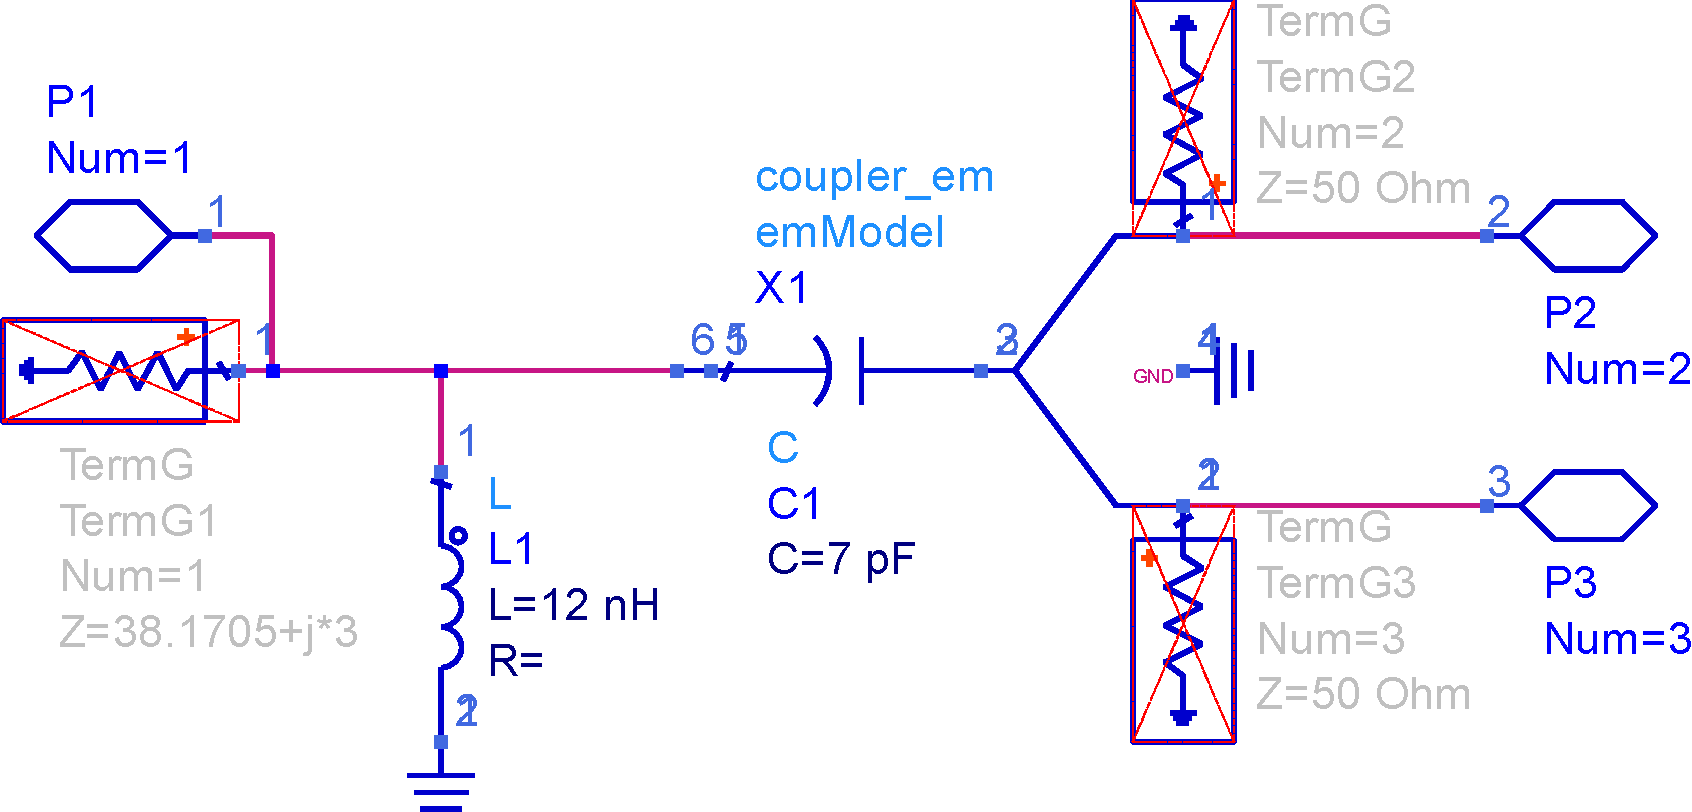
\includegraphics[width=\textwidth]{coupler-match.pdf}
		\caption{}%
		\label{fig:coupler-match}
	\end{subfigure}
	\caption{%
		(а) Топология и 
		(б) схема согласования делителя
	}%
	\label{fig:coupler-em-sch}
\end{figure}

На Рисунке \ref{fig:IPL-coupler-results} показаны результаты моделирования входного тракта с учетом делителя мощности.

\begin{figure}[H]
	\centering
	\begin{subfigure}[c]{0.49\textwidth}
		\centering
		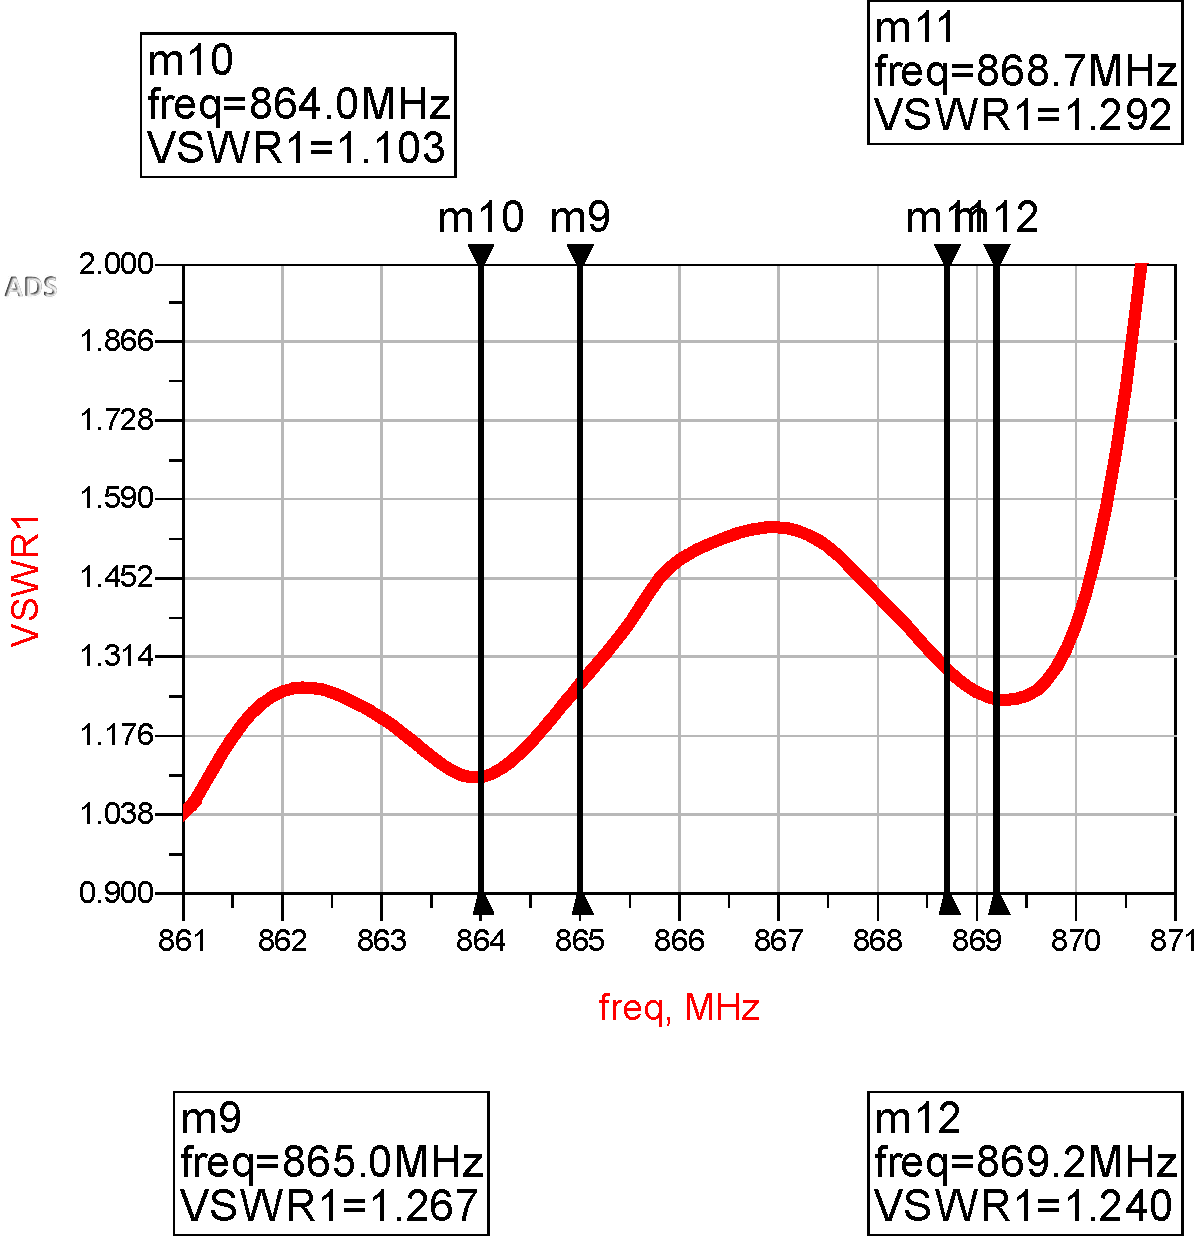
\includegraphics[width=\textwidth]{IPL-coupler-VSWR.pdf}
		\caption{}%
		\label{fig:IPL-coupler-VSWR}
	\end{subfigure}
	\hfill
	\begin{subfigure}[c]{0.49\textwidth}
		\centering
		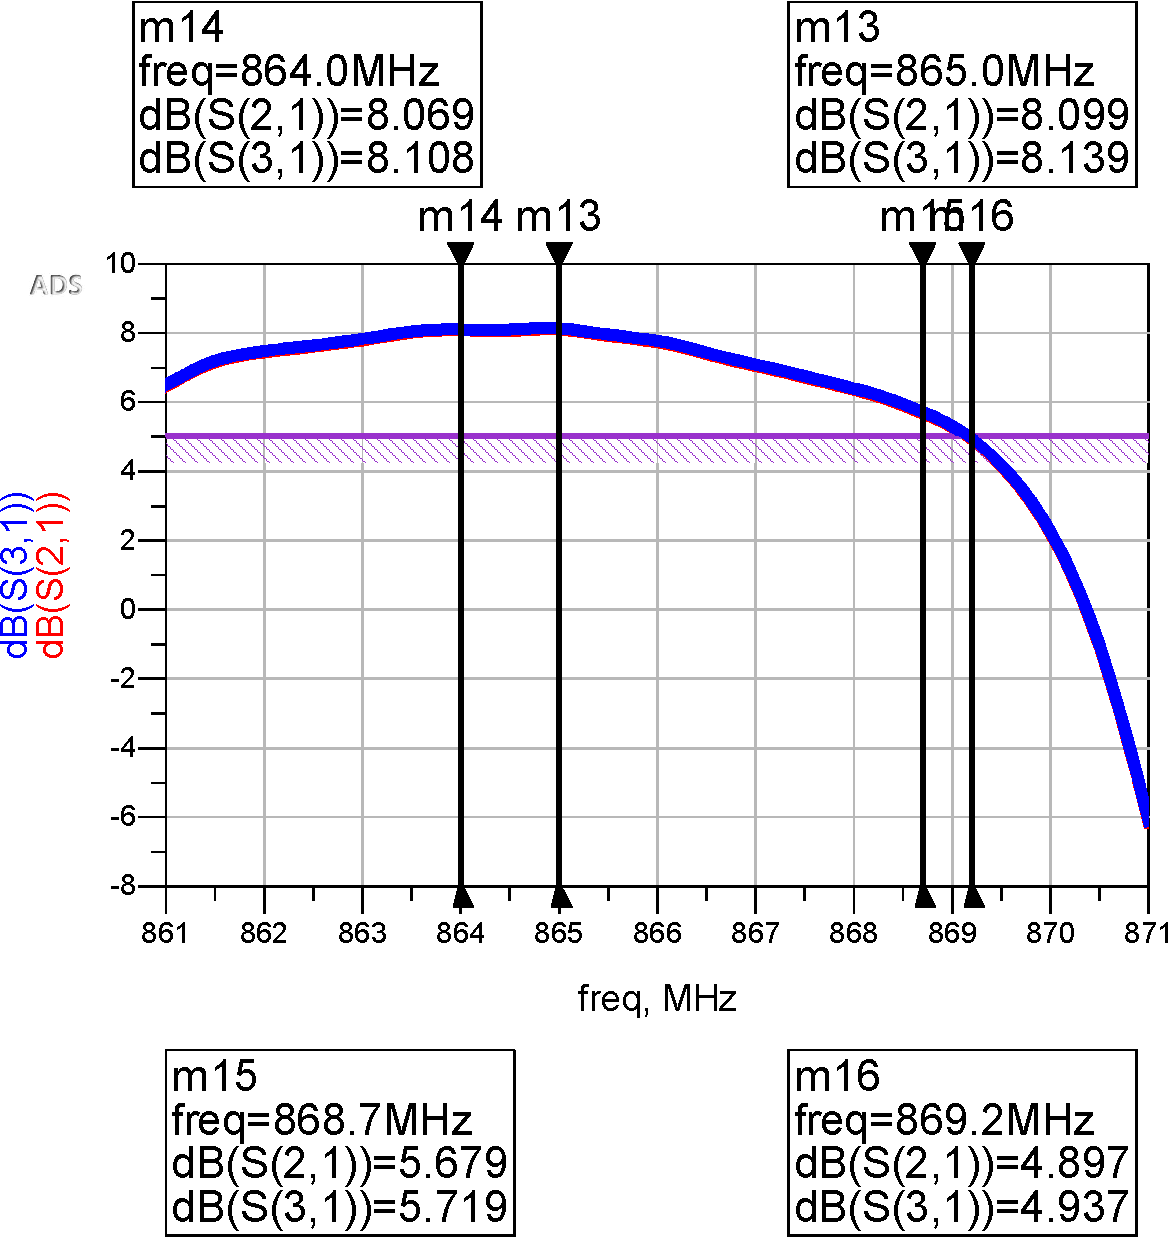
\includegraphics[width=\textwidth]{IPL-coupler-trans.pdf}
		\caption{}%
		\label{fig:IPL-coupler-trans}
	\end{subfigure}
	\caption{%
		(а) Топология и 
		(б) схема согласования делителя
	}%
	\label{fig:IPL-coupler-results}
\end{figure}

\subsection{Составление библиотек ЭКБ.}

Дальнейшая работа будет проводиться в Altium Designer. На основе документации производителей и требований ГОСТ 2.710-81 и ГОСТ 2.743-91 составлены библиотеки УГО и посадочных мест используемых компонентов.

Составленные библиотеки находятся в репозитории проекта в соответствующем разделе.

\subsection{Разработка электрической схемы.}

Основываясь на результатах проведенного моделирования и ориентируясь на рекомендации производителей в соответствии с ГОСТ 2.702-2011 была разработана электрическая принципиальная схема устройства. Схема разбита на несколько листов.

\begin{figure}[H]
	\centering
	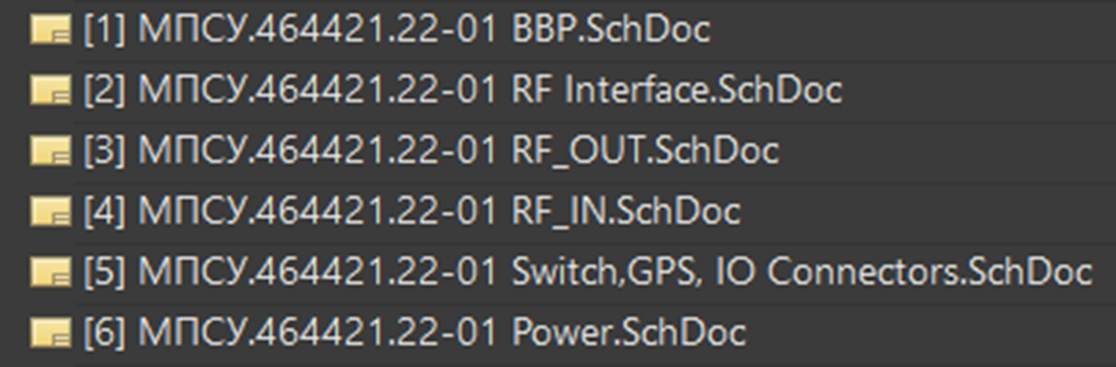
\includegraphics[width=0.6\textwidth,keepaspectratio]{bs-sch-grouping.png}
	\caption{Разбиение схемы электрической принципиальной}%
	\label{fig:bs-sch-grouping}
\end{figure}

Эскиз листа со схемой приёмного канала показан на Рисунке \ref{fig:bs-sch-rf-in}

\begin{figure}[H]
	\centering
	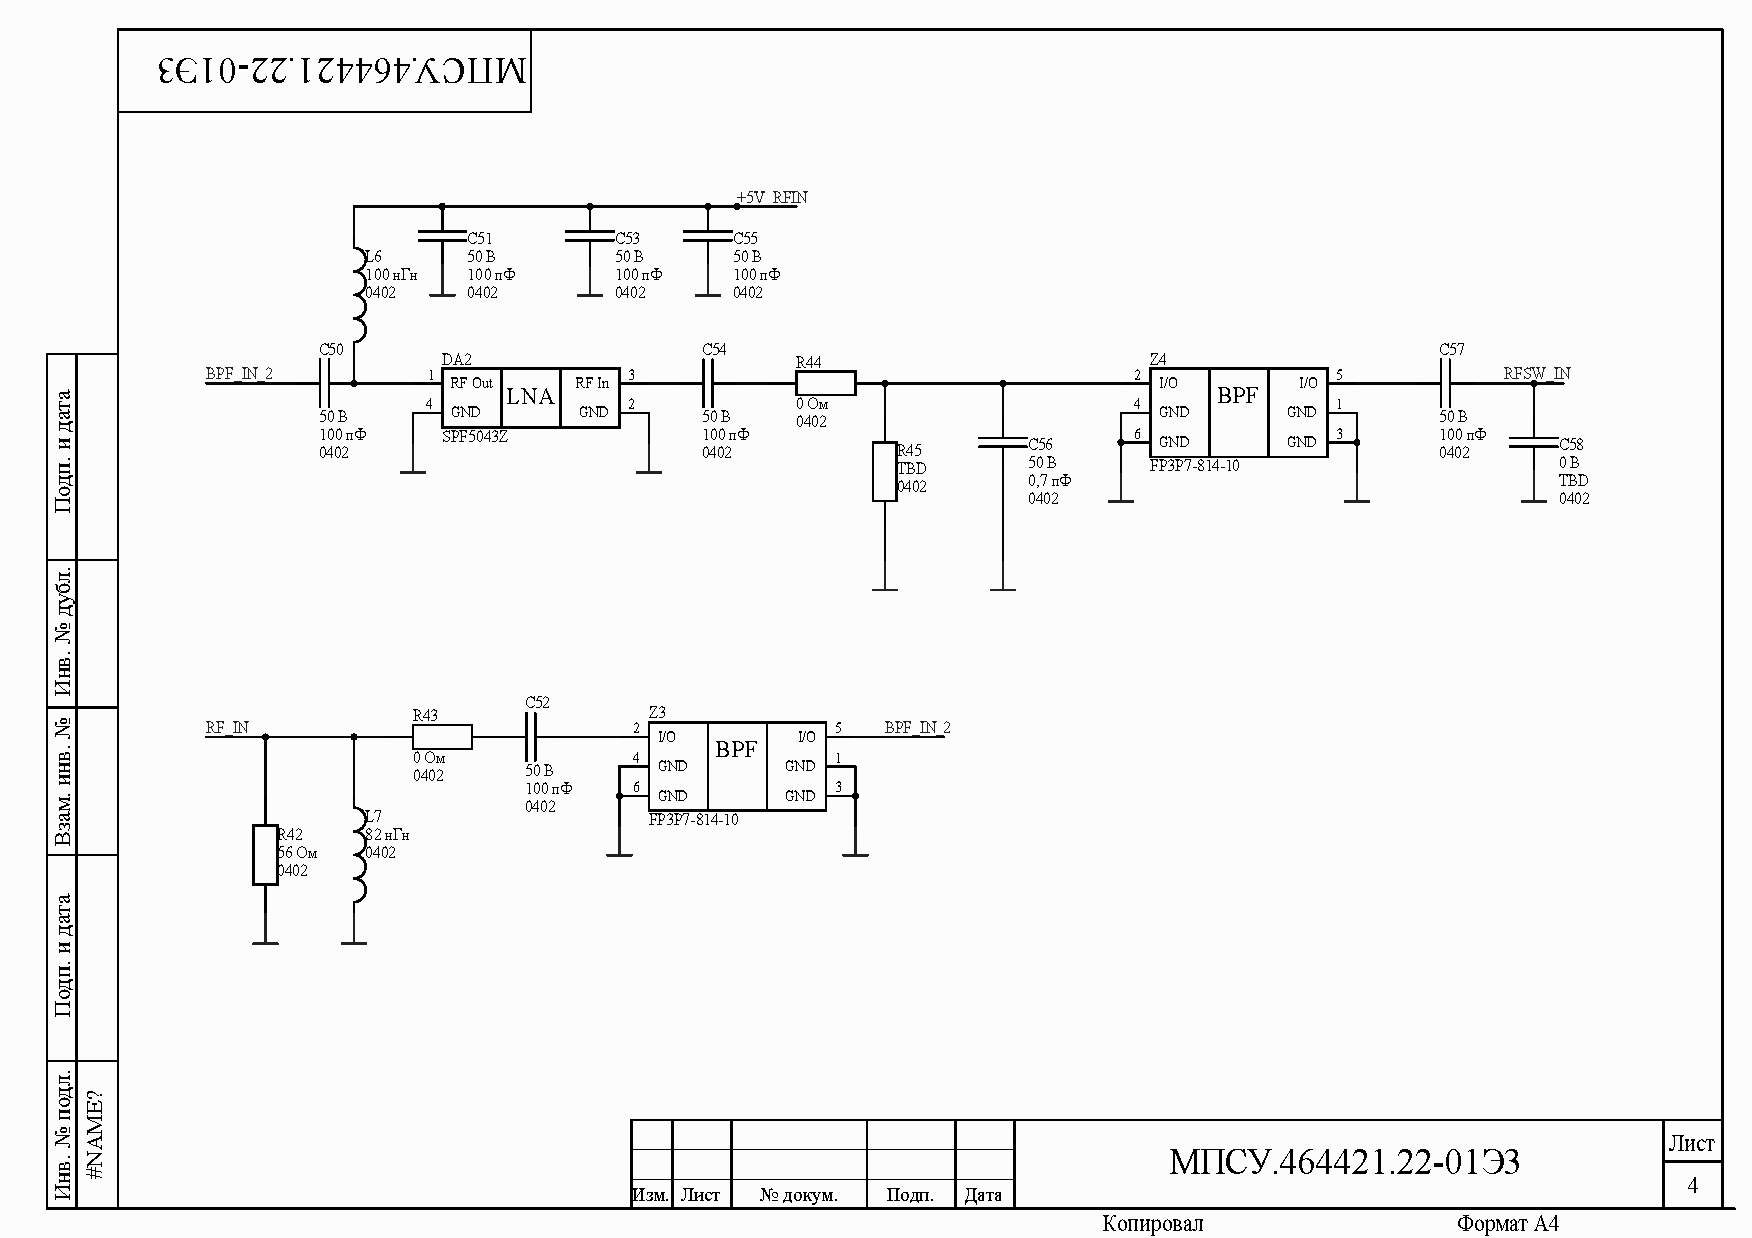
\includegraphics[width=\textwidth,keepaspectratio]{bs-sch-rf-in.pdf}
	\caption{Эскиз одного из листов Э3 на БС.}%
	\label{fig:bs-sch-rf-in}
\end{figure}

Более подробно про экспорт документации будет рассказано в главе \ref{sect:project-docs}.

\subsection{Проектирование топологии.} \label{sect:bs-topology}

На основании схемы электрической принципиальной, с использованием составленных ранее библиотек и с учетом возможностей современных производителей печатных плат была спроектирована топология печатной платы устройства. На Рисунке \ref{fig:bs-stackup} показано отображение стека платы в Altium Designer.

\begin{figure}[H]
	\centering
	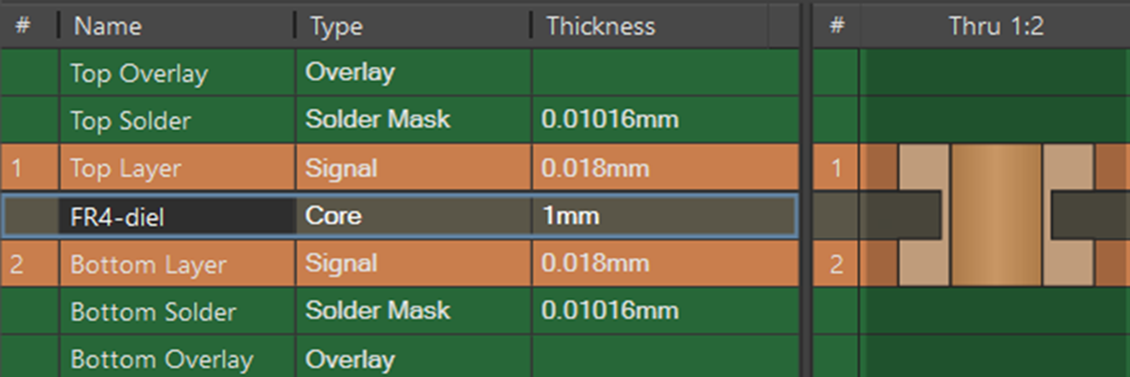
\includegraphics[width=0.7\textwidth,keepaspectratio]{bs-stackup.png}
	\caption{Стек печатной платы БС}%
	\label{fig:bs-stackup}
\end{figure}

На следующих рисунках показано отображение основной информации о печатной плате и печатном узле БС.

\begin{figure}[H]
	\centering
	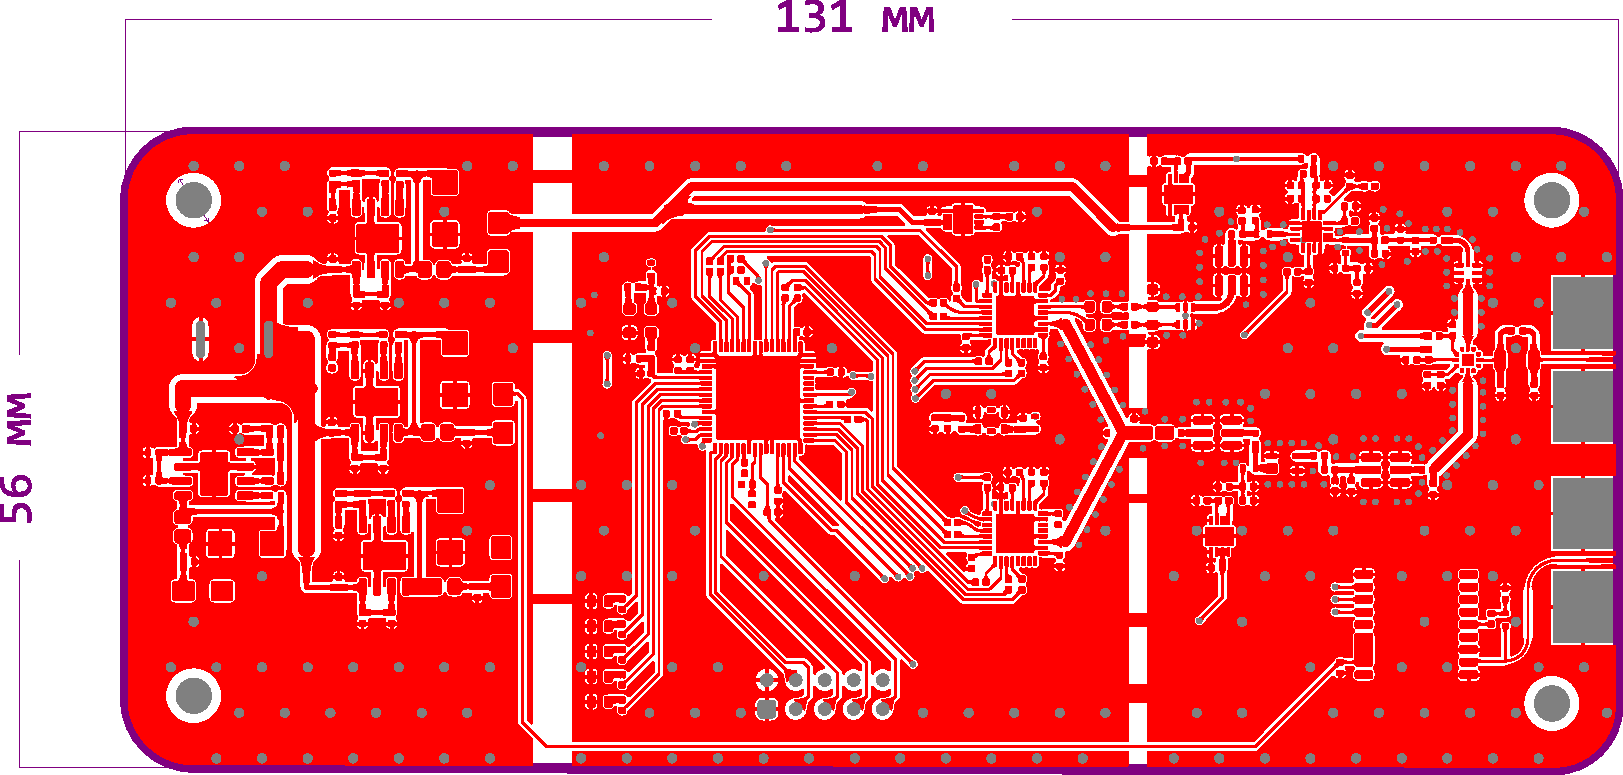
\includegraphics[width=\textwidth,keepaspectratio]{BS-Top Layer.pdf}
	\caption{Топология верхнего слоя}%
\end{figure}

\begin{figure}[H]
\centering
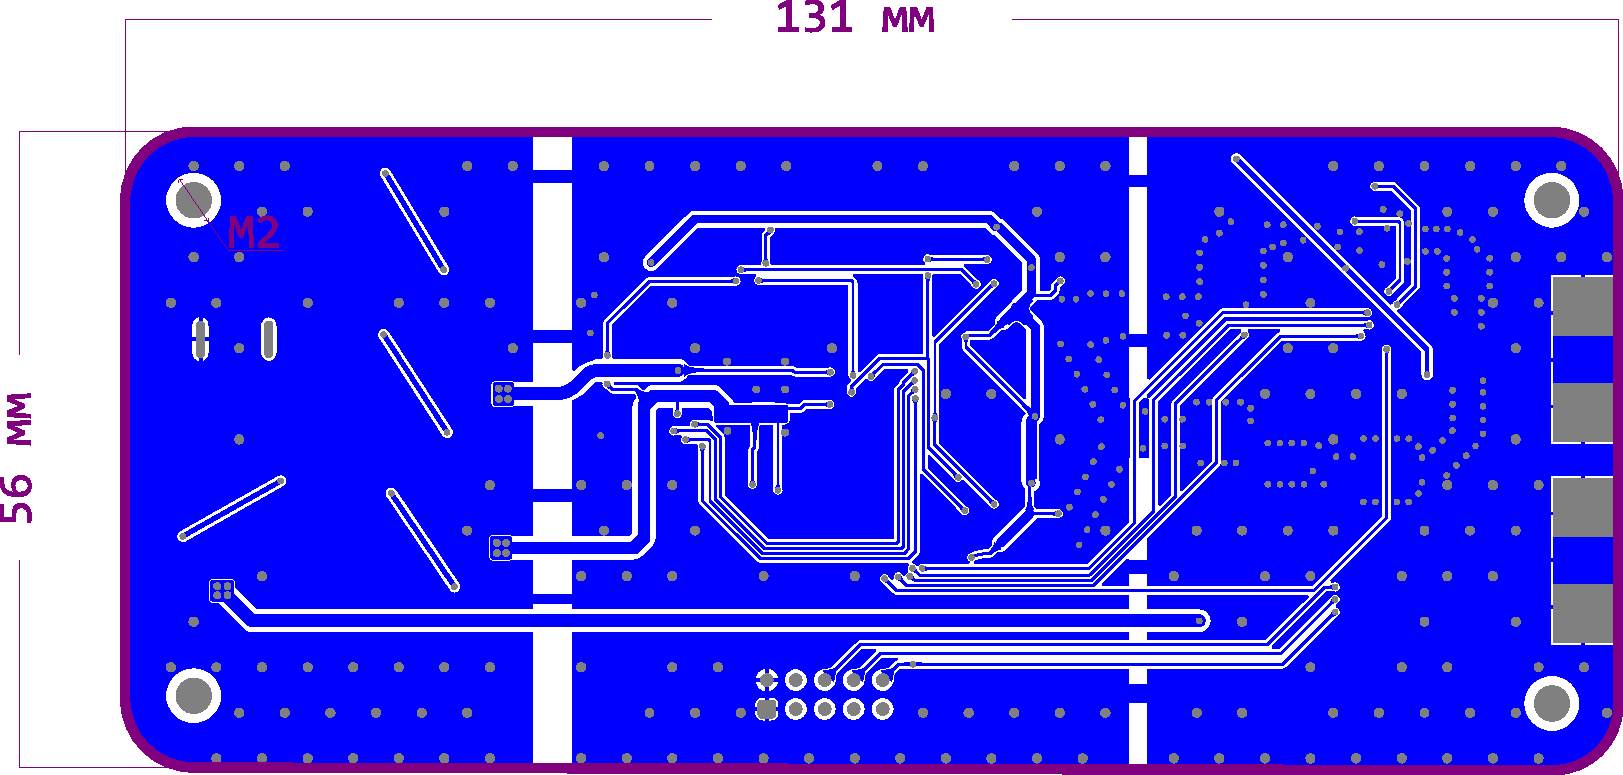
\includegraphics[width=\textwidth,keepaspectratio]{BS-Bottom Layer.pdf}
\caption{Топология нижнего слоя}%
\end{figure}


\begin{figure}[H]
	\centering
	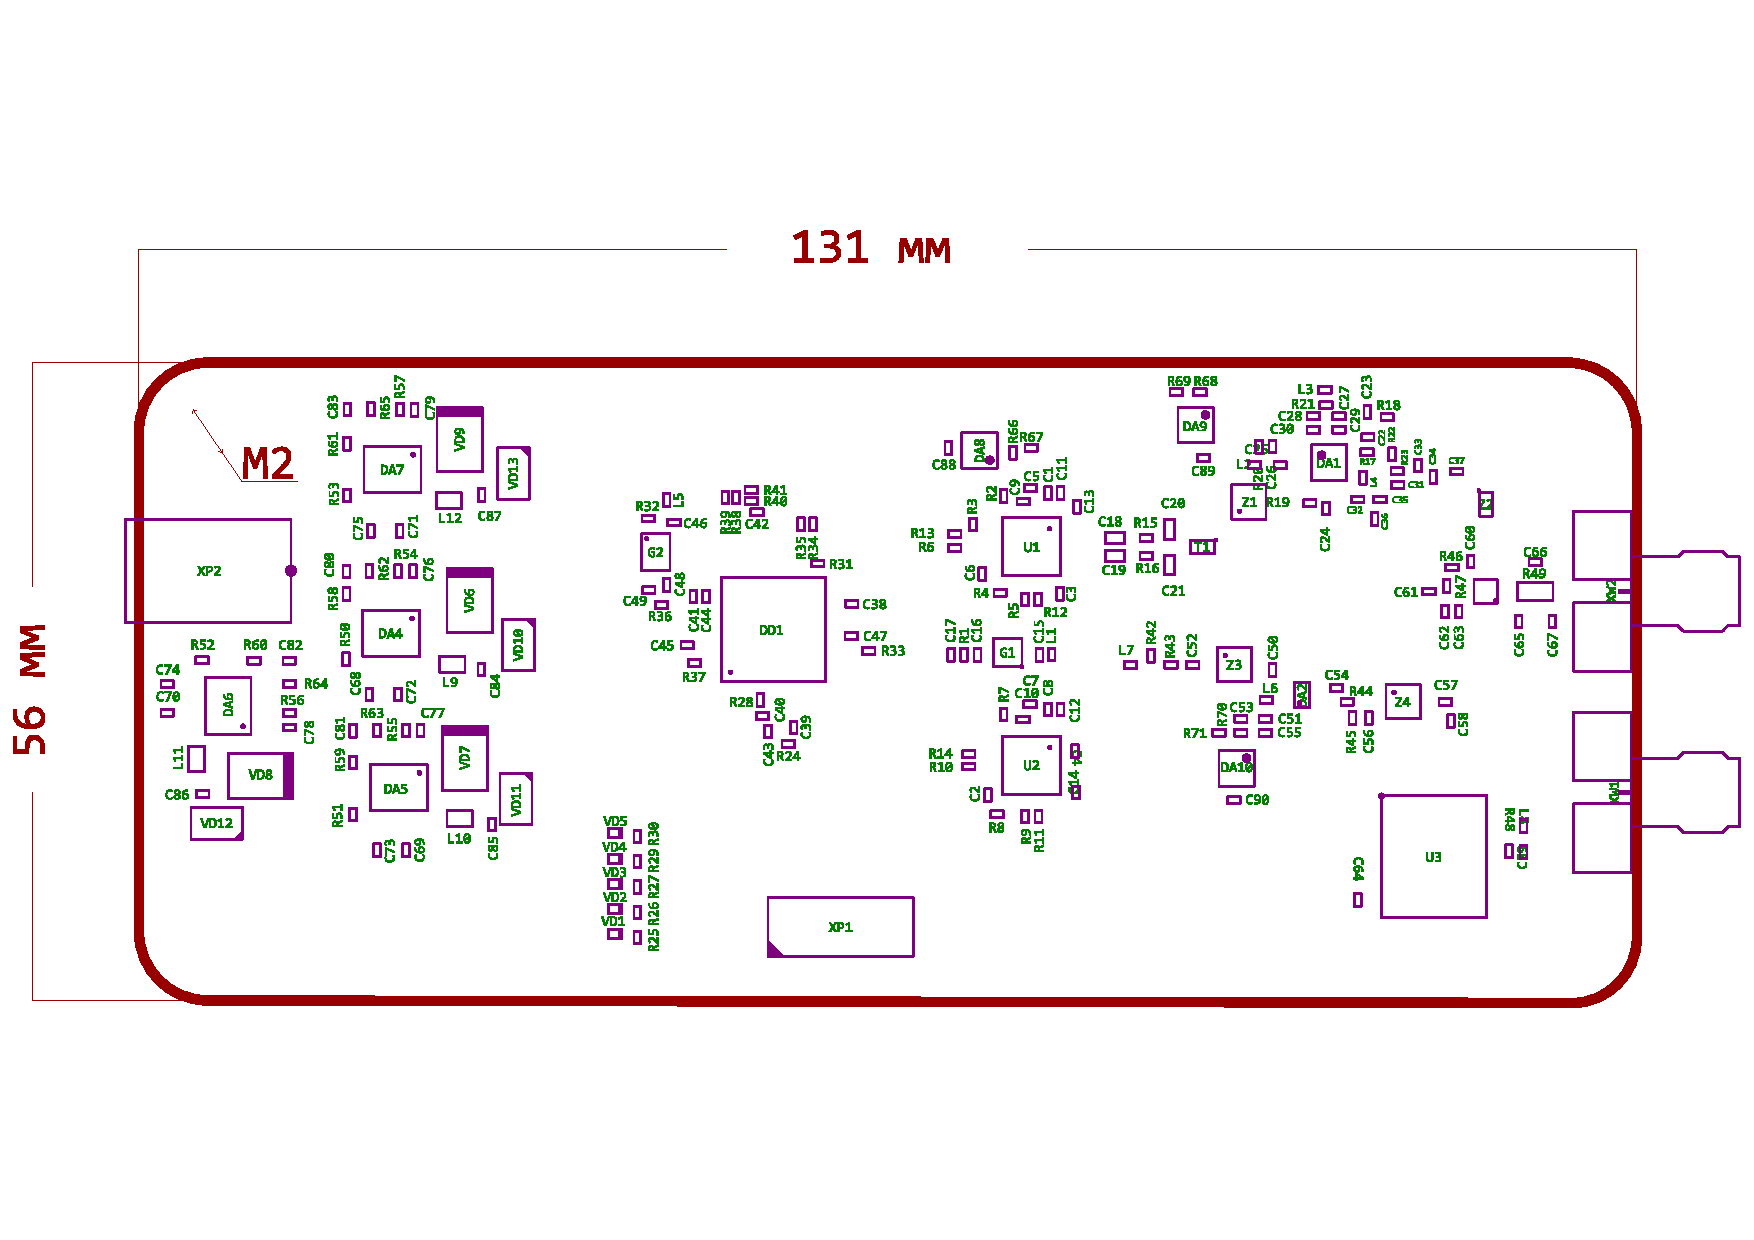
\includegraphics[width=\textwidth,keepaspectratio]{BS-Assembly Drawing.pdf}
	\caption{Эскиз сборочного чертёжа}%
\end{figure}

\subsection{Трёхмерная модель и поддерживающая рамка.}

Altium Designer позволяет отображать фотореалистичные модели разработанных печатных плат. С учетом этого, ещё на стадии формирования библиотек были созданы 3D модели компонентов. Итоговый вид платы можно увидеть на Рисунке \ref{fig:3D-Board}.

\begin{figure}[H]
	\centering
	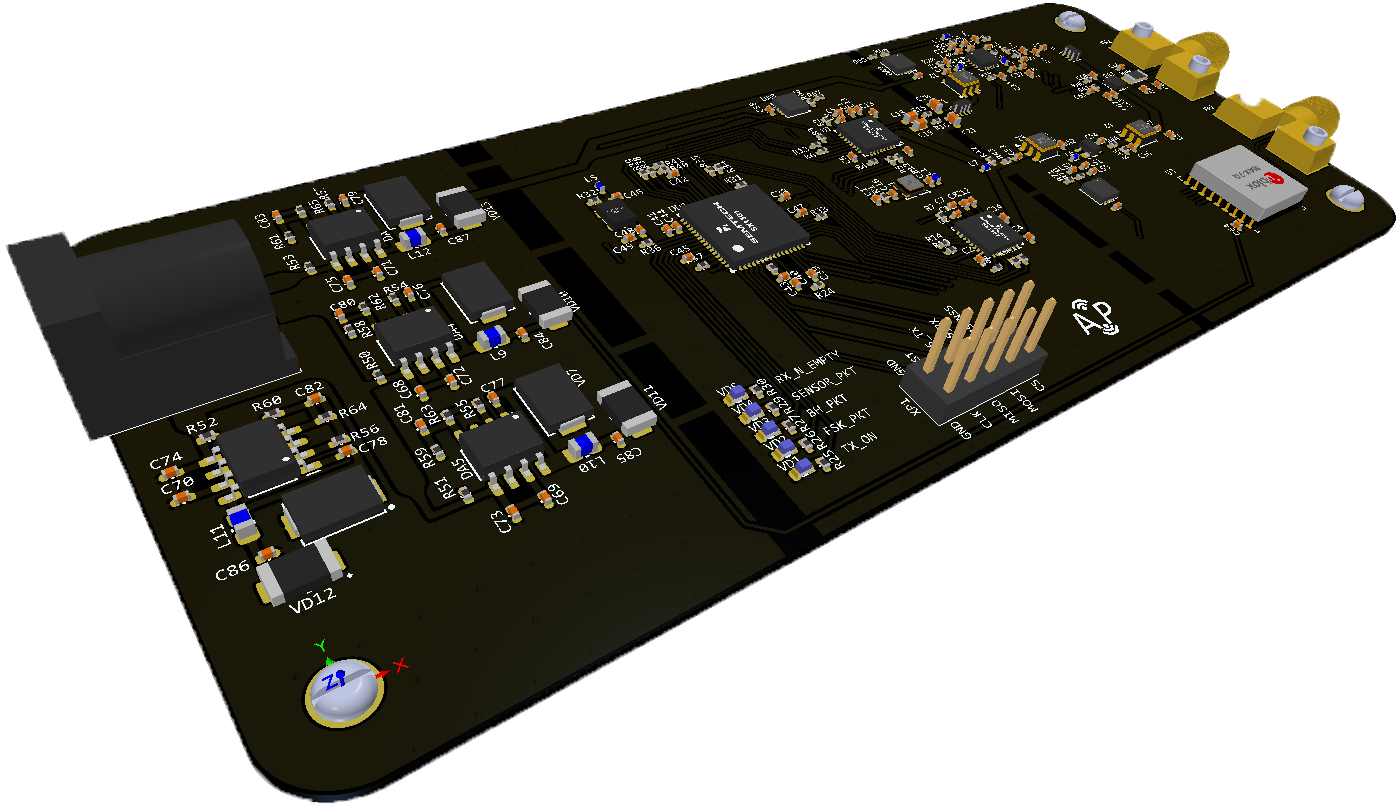
\includegraphics[width=\textwidth,keepaspectratio]{3D-Board.png}
	\caption{трехмерная модель платы, изометрический вид.}%
	\label{fig:3D-Board}
\end{figure}

Также для удобства эксплуатации модуля была разработана поддерживающая рамка, показанная на Рисунке \ref{fig:BS-Frame}. Итоговая сборка показана на Рисунке \ref{fig:bs-3d-framed}.

\begin{figure}[H]
	\centering
	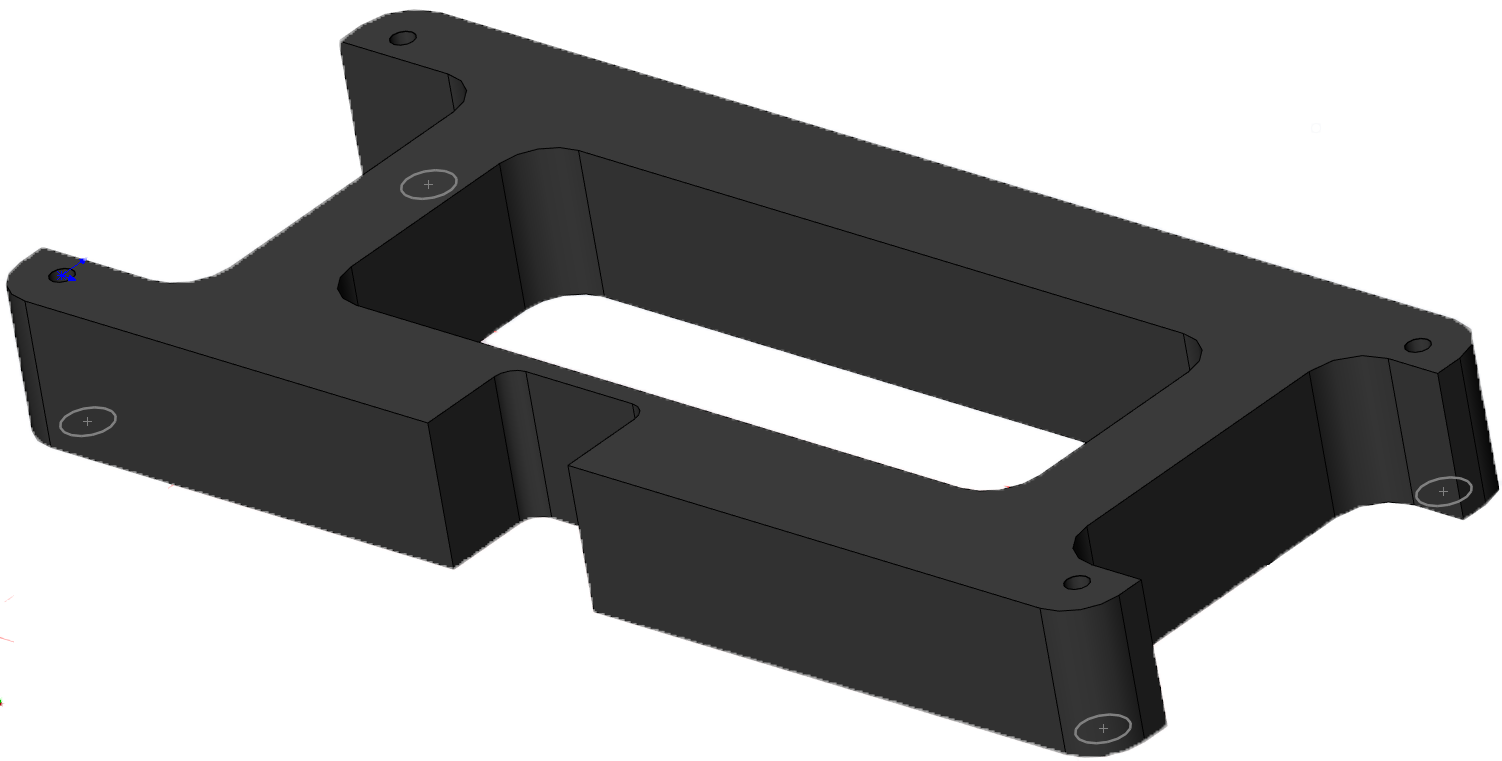
\includegraphics[width=\textwidth,keepaspectratio]{BS-Frame.png}
	\caption{трёхмерная модель рамки, изометрический вид сверху.}%
	\label{fig:BS-Frame}
\end{figure}

\begin{figure}[H]
	\centering
	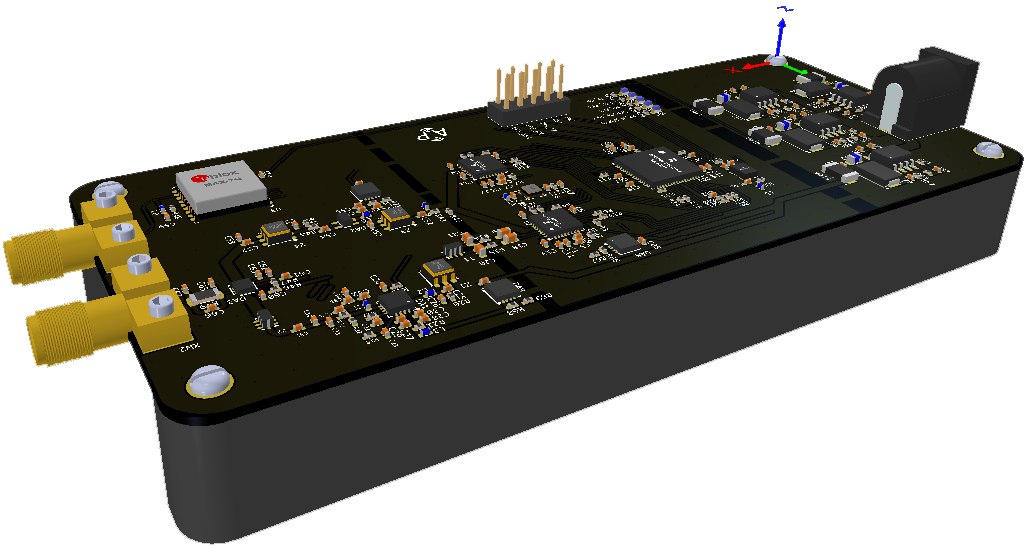
\includegraphics[width=\textwidth,keepaspectratio]{bs-3d-framed.png}
	\caption{трехмерная модель сборки. Изометрический вид сверху.}%
	\label{fig:bs-3d-framed}
\end{figure}


\subsection{Разработка платы измерения параметров усилителя.} \label{sect:bs-oa-mes}

Как упоминалось в Главе \ref{sect:bs-topology}, для получения более точных характеристик усилителя, была разработана плата измерения. Электрическая схема включения усилителя аналогична схеме включения в основном проекте – по входу и выходу установлены универсальные схемы согласования - набор из двух последовательных и двух параллельных компонентов. Этого набора достаточно для согласования большинства устройств.

\begin{figure}[H]
	\centering
	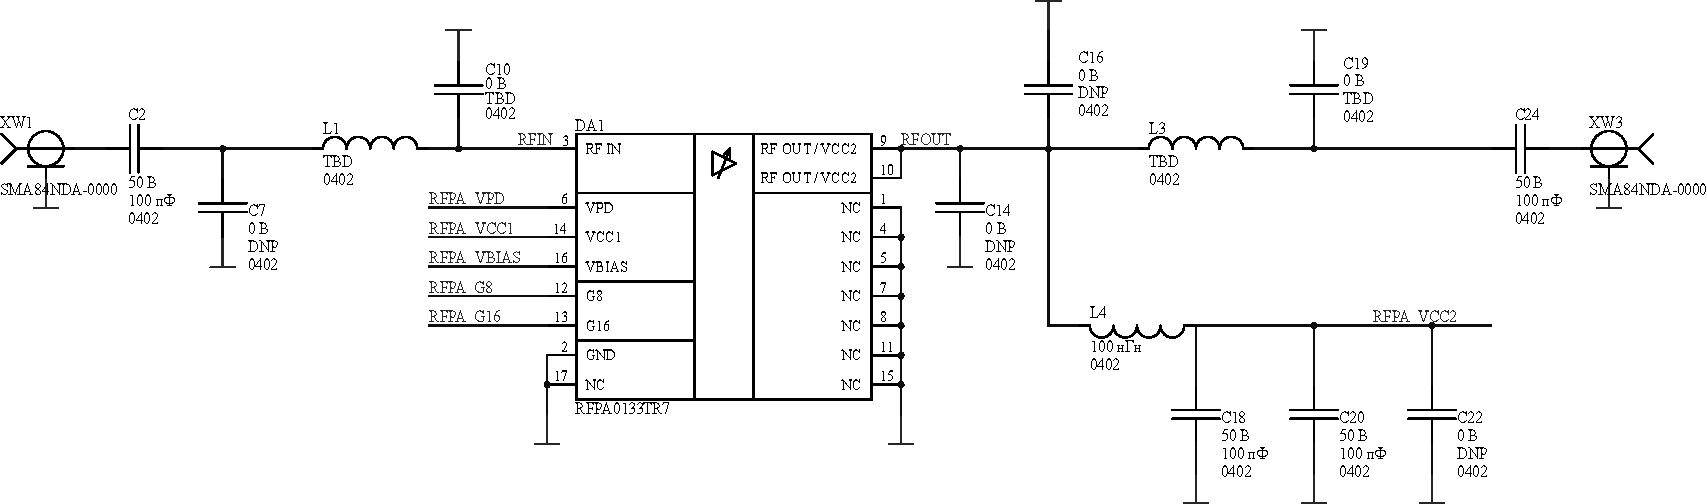
\includegraphics[width=\textwidth,keepaspectratio]{pa-measuring-sch.pdf}
	\caption{электрическая схема включения УМ}%
	\label{fig:pa-measuring-sch}
\end{figure}

 Дополнительно была создана линия для калибровки средств измерения. Она является полной копией основной линии за исключением измеряемого компонента.

\begin{figure}[H]
	\centering
	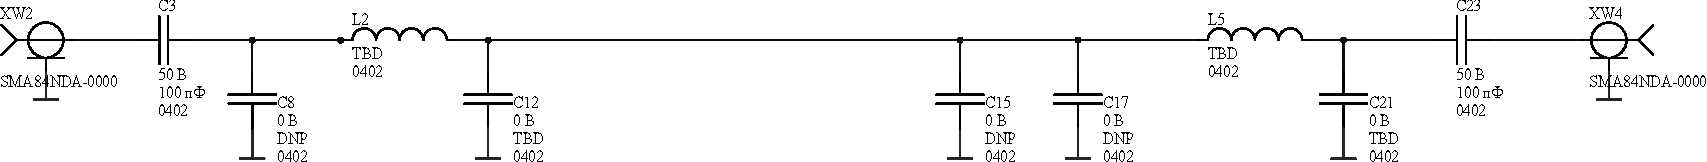
\includegraphics[width=\textwidth,keepaspectratio]{pa-measuring-cal-line-sch.pdf}
	\caption{линия для калибровки}%
	\label{fig:pa-measuring-cal-line-sch}
\end{figure}

Для уменьшения количества неоднородностей ширину линии была выбрана равной ширине контактных площадок микросхемы усилителя. 

Чтобы обеспечить достоверность измерения не только амплитуды, но и фазы, нужно удостовериться в полной идентичности цепи калибровки и цепей включения компонента. Для удовлетворения данного требования выходные и выходные цепи линии измерения были скопированы и перенесены на топологическом уровне. 

Внешний вид разработанной платы показан на Рисунке \ref{fig:pa-measuring-topview}. Сверху находится измерительная линия, снизу – линия калибровки.

\begin{figure}[H]
	\centering
	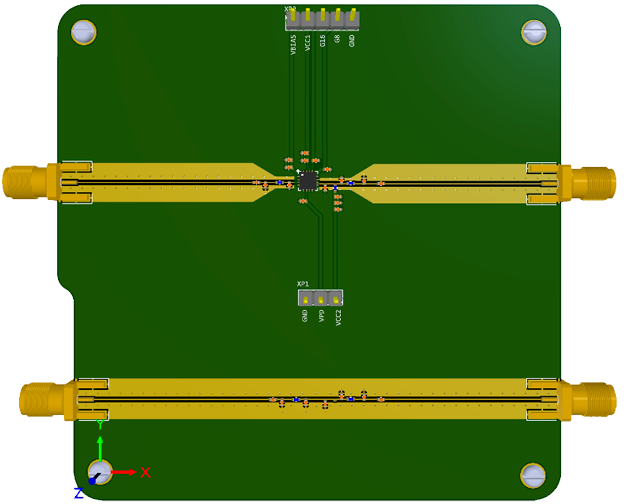
\includegraphics[width=\textwidth,keepaspectratio]{pa-measuring-topview.png}
	\caption{3D модель измерительной платы. Вид сверху.}%
	\label{fig:pa-measuring-topview}
\end{figure}



